
\documentclass[10pt]{report}

\usepackage{csquotes}
\usepackage{graphicx}
\usepackage{color}
\usepackage[spanish]{babel}
\usepackage{amsmath,amsfonts,amssymb,amsthm}
\usepackage{fontenc,url,path}
\usepackage{hyperref}
\usepackage{float}
\usepackage{bookmark}
\usepackage{todonotes}

\usepackage{geometry} % Add this line
\geometry{margin=1.4in} % Adjust margins as needed

\usepackage{biblatex} %Imports biblatex package
\addbibresource{referencias.bib}

\hypersetup{colorlinks,
            urlcolor=blue,
            citecolor=blue}

\graphicspath{{figuras/}}

% layout pars
\setlength{\parindent}{0pt}
\setlength{\arraycolsep}{2pt}
\setlength{\parskip}{3pt}
\vfuzz2pt % don't report over-full v-boxes if over-edge is small
\hfuzz2pt % don't report over-full h-boxes if over-edge is small

% commands
\newcommand{\intro}[1]
  {{\normalsize\textsf{#1}}}

\newcommand{\blankpage}%
  {\newpage
   \null\vfill\eject}

% customized 'description' environment
\renewcommand{\descriptionlabel}[1]%
	{\hspace{\labelsep}\textsf{#1}}

% text commands
\def\etal{et al.}
\def\ie{i.e}
\renewcommand\spanishtablename{Tabla}

% math commands
\DeclareMathOperator{\E}{E}
\DeclareMathOperator{\Cov}{Cov}
\DeclareMathOperator{\Cor}{Cor}
\DeclareMathOperator{\var}{var}
\DeclareMathOperator{\abs}{abs}
\DeclareMathOperator{\argmax}{arg\,max}
\DeclareMathOperator{\argmin}{arg\,min}
\DeclareMathOperator{\blkdiag}{blc\,diag}
\DeclareMathOperator{\diag}{diag}
\DeclareMathOperator{\rd}{d}
\DeclareMathOperator{\GIF}{GIF}
\let \max \relax
\DeclareMathOperator{\max}{max}
\let \min \relax
\DeclareMathOperator{\min}{min}
\DeclareMathOperator{\nullity}{nulidad}
\let \Pr \relax
\DeclareMathOperator{\Pr}{P}
\DeclareMathOperator{\rk}{rg}
\let \SS \relax
\DeclareMathOperator{\SS}{SS}
\DeclareMathOperator{\SSD}{SSD}
\DeclareMathOperator{\tr}{tr}
\let \vec \relax
\DeclareMathOperator{\vec}{vec}
\DeclareMathOperator{\vech}{vech}
\DeclareMathOperator{\vecp}{vecp}
\def\half{{\textstyle\frac{1}{2}}}
\def\Cset{\mathbb{C}}
\def\Hset{\mathbb{H}}
\def\Nset{\mathbb{N}}
\def\Qset{\mathbb{Q}}
\def\Rset{\mathbb{R}}
\def\Zset{\mathbb{Z}}
\def\D{\mathsf{D}}
\def\H{\mathsf{H}}
\newcommand{\bt}[1]{\ensuremath{\mathbf{#1}}}  % bold text
\newcommand{\bm}[1]{\mbox{\boldmath $#1$}}     % bold math
\newcommand{\bc}[1]{\ensuremath{\mathcal{#1}}}  % bold text
\newcommand{\what}[1]{\widehat{#1}}             % shortcut for \widehat
\newcommand{\C}{\textsf{C}}
\newcommand{\Fortran}{\textsc{Fortran}}
\newcommand{\R}{\mathbb{R}}
\newcommand{\s}{\textsf{S}}
\newcommand{\Splus}{\textsc{S-Plus}}

% Theorems -------------------------------------------------------------
\theoremstyle{plain}
\newtheorem{fact}{Hecho}
\newtheorem{thm}{Teorema}[chapter]
\newtheorem{cor}[thm]{Corolario}
\newtheorem{lem}[thm]{Lema}
\newtheorem{property}[thm]{Propiedad}
\theoremstyle{definition}
\newtheorem{defn}{Definici\'{o}n}[chapter]
\newtheorem{asump}{Supuesto}[chapter]
\newtheorem{prop}{Proposici\'{o}n}[chapter]
\newtheorem{result}{Resultado}[chapter]
\theoremstyle{remark}
\newtheorem{rem}{Observaci\'{o}n}[chapter]
\newtheorem{example}{Ejemplo}[chapter]

\title{{\LARGE\textbf{T\'opicos de Modelaci\'on Estad\'istica}} \\[0.8ex]
    {\large\textbf{Notas de Clase MAT-305: M\'etodos Estad\'isticos}}}

\author{Felipe Osorio}

\hyphenation{ob-te-ne-mos
    pro-ba-bi-li-dad
    si-guien-tes
    va-rian-za}

\begin{document}

\DeclareGraphicsExtensions{.epsi.gz,.epsi,.eps.gz,.eps,.ps,.ps.gz}

% ----------------------------------------------------------------------

% ---------------------------------------------------------------------------------------
\thispagestyle{empty}

\begin{center}
%~\\
%~\\
\large \textbf{UNIVERSIDAD T\'ECNICA FEDERICO SANTA MAR\'IA}

\vspace{3mm}

\normalsize DEPARTAMENTO DE MATEM\'ATICA
\vspace{35mm}

\Large {\bf An\'alisis de Imagenes transformadas con Box-Cox}

\vspace{35mm}

\normalsize Memoria de T\'itulo presentada por

\vspace{2mm}

\large{\textbf{Fabi\'an Castellano N\'u\~nez}}

\vspace{10mm}

\normalsize como requisito parcial para optar al t\'itulo de

\vspace{2mm}

\textbf{Ingeniero Civil Matem\'atico}

\vspace{15mm}

Profesor Gu\'ia

\vspace{2mm}

Dr. Ronny Vallejos S.

\vspace{5mm}

Marzo, 2024.

\end{center}
\blankpage
\chapter*{Agradecimientos.}

Primero que todo, debo agradecer a las dos m\'ujeres m\'as importantes de mi vida, mi madre Jessicca y mi pareja Noem\'i, sin su amor y apoyo incondicional me hubiera sido imporsible llegar tan lejos. No hay palabras que pueda escribir para expresar todo lo que les debo.

Junto con ellas debo mencionar a mi Lela Rosa, a quien no llamo por telefono tanto como deber\'ia, pero siempre esta presente cuandio m\'as la necesito. Y también a Claudio, con cuyo apoyo, sin dudarlo, siempre puedo contar.

Gracias a mis amigos, en particular a Gustavo, Ricardo, y Bruno, por siempre estar disponibles para ayudar, y recordarme que el final no está tan lejos. Junto con ellos quiero dar las gracias a toda la \textit{gente de mate} que me ha acompa\~nado durante estos a\~nos.

Agradezco tambi\'en a mi profesor gu\'ia, Dr. Ronny Vallejos, no solo por el apoyo y la direcci\'on que me dió durante el trabajo, sino por la gran cantidad paciencia y cariño que me entreg\'o durante todo el proceso. Además debo agradecer todos los profesores, tanto del departamento de matem\'aticas como otros, quienes me han guiado durante estos a\~nos. Tambi\'en agradezco a Andrea y Astrik, por siempre estar disponibles con una sonrisa y una soluci\'on para todos los problemas que me llevaron a su oficina.


No puedo olvidar dar las gracias a la gente de TallerCaf\'e; Gabriela, Camilo, y Monserrat, por siempre estar para entregar animos, y por aguantar mis quejas sobre este trabajo por m\'as tiempo de el que me es c\'omodo admitir.

Por \'ultimo, agradezco al mi familia, que a pesar de la distancia su apoyo es sentido y apreciado. Sin todo su todo su amor y su apoyo, no hubiera sido posible superar todos los obst\'aculos que se me han presentado durante estos a\~nos.

Gracias a todos ustedes, y a todos los que no mencion\'e, agradezco poder terminar esta et\'apa de mi vida con gente tan maravillosa a mi lado.
% show outile 
\setcounter{tocdepth}{1}
\tableofcontents
\blankpage
% ---------------------------------------------------------------------------------------
\chapter{Introducci\'on}\label{chap1}

En el an\'alisis de datos, es com\'un verse enfrentado con datos problem\'aticos, valores faltantes, datos at\'ipicos, o datos que no distribuyan de forma normal. En el caso de este \'ultimo, es com\'un aplicar transformaciones a los estos para que su distribuci\'on se asemeje a una Normal. Una de las transformaciones m\'as comunes para lograr esto es la transformaci\'on de Box-Cox, la cual busca a travez de un problema de optimizaci\'on, encontrar el valor de $\lambda$ que mejor ajuste los datos a una distribuci\'on Normal. Esta transformaci\'on suele aplicase sobre  vectores unidimensionales, y no ha sido extendida a matrices $d$-dimensionales en las que existe corrlaciones de adyacencia, excepto en una cantidad muy reducida de trabajos, en los que destacan Lee et. al. \textit{(MR Image Segmentation Using a Power Transformation Approach)}\cite{lee2009mr}, y Bicego y Baldo \textit{(Properties of the Box-Cox Transformation for Pattern Classification)}\cite{bicego2016}. 

En el primero se trata el problema de segmentaci\'on de imagenes de resonancia magn\'etica, y utlizan la transformaci\'on simplemente aplananado la matriz de la imagen. En el segundo se estudian distintas propiedes de la transformaci\'on de Box-Cox sobre ima\'agenes, en particular para clasificaci\'on de patrones. En el segundo trabajo, se propone algo interesante, utilizar el histograma de la imagen para encontrar el valor de $\lambda$ que mejor ajuste los valores de este a una distribuci\'on normal. Dado este interes por aplicar la transformaci\'on de Box-Cox a im\'agenes, y la falta de trabajos en esta direcci\'on, nos interesa estudiar la relaci\'on que existe entre la transformaci\'on de Box-Cox y la im\'agen original de donde proviene,

Recordemos que esta transformaci\'on es no lineal, por lo que nos interesa utilziar m\'etodos de comparaci\'on que nos permitan detectar relaciones no lineales entre las variables. Por esto es que comenzaremos el trabajo en el Cap\'itlo \ref{chap2} dos m\'etodos de comparaci\'on, en particular estudiaremos el \textit{Maximal Information Coefficient} o MIC, y el \textit{Distance Correlation} o dCor, donde revisaremos como se define cada uno, y como podemos calcularlo, adem\'as de algunos ejemplos de su aplicaci\'on.

Continuaremos en el Cap\'itlo \ref{chap3} revisando como trabajamos con im\'agenes, su interpretaci\'on como matrices, y como procederemos a aplicar m\'etodos de comparaci\'on sobre estas imagenes. Adem\'as revisaremos el banco de imagenes que utilizaremos para realizar los experimentos. Luego, en el Cap\'itlo \ref{chap4} procederemos a estudiar la tranformaci\'on de Box-Cox, su definici\'on, como podemos aplicarla sobre im\'agenes, y discutiremos distintos m\'etodos para la obtenci\'on del valor $\lambda$. 

Finalmente en el Cap\'itlo \ref{chap5}, ya con todo esto cubierto, procederemos a realizar experimentos num\'ericos, en los que aplicaremos la transformaci\'on de Box-Cox sobre im\'agenes, y compararemos la im\'agen original con la transformada, utilizando los m\'etodos de comparaci\'on estudiados en el cap\'itulo \ref{chap2}.

El objetivo de este trabajo es estudiar la relaci\'on que existe entre la transformaci\'on de Box-Cox y la im\'agen original de donde proviene, en particular para distintas formas de encontrar valores de $\lambda$, y para distintos tipos de im\'agenes. Adem\'as de proponer un m\'etodo para encontrar el valor de $\lambda$. Junto con esto, tambie\'en se explora el concepto de comparaci\'on de ima\'agenes, proponiendo un m\'etodo novedoso para comparar im\'agenes que no se basa en la comparaci\'on de pixeles, sino que en la comparaci\'on de la distribuci\'on de los valores de los pixeles, utilizando el histograma de la imagen como base para la comparaci\'on.
\blankpage
% ---------------------------------------------------------------------------------------
\chapter{Análisis Estadistico y Procesamiento de Imagenes }\label{chap2}


% ---------------------------------------------------------------------------------------
\section{Definiciones previas}


\blankpage
\chapter{\textit{Maximal Information Coeficient}}

La Coeficiente de Informaci\'on m\'axima (conocido como MIC por sus siglas en ingl\'es), es una medida estad\'istica propuesta por Reshef et al. en su paper "Detecting Novel Associations in Large Data Sets" \cite{Reshef2011}. Este coeficiente fue creado en el contexto de la ciencia generadora de hip\'otesis, en la cual los conjuntos de datos se utilizan para ayudar a los investigadores a formular nuevas hip\'otesis en lugar de probar las existentes. En este enfoque, se utilizan medidas de dependencia, que son estad\'isticas empleadas para evaluar pares de variables candidatas. Estos avances en el campo de analisis de datos nos han entregado muchas herramientas, tanto para la comparaci\'on de datos en si mismos, junto con formas de evaluar estas medidas en si mismas.

Sea $\hat\varphi$ una medida de dependencia, una forma de medir la utilidad de esta es la \textit{potencia contra la independencia}, i.e., la capacidad de prueba de independencia basada en $\hat\varphi$ para detectar varios tipos de relaciones no triviales. Este es un objetivo importante para conjuntos de datos que tienen muy pocas relaciones no triviales, o solo relaciones muy d\'ebiles que son dif\'iciles de detectar. Sin embargo, a menudo el n\'umero de relaciones declaradas estad\'isticamente significativas por una medida de dependencia supera con creces el n\'umero de relaciones que luego se pueden explorar m\'as a fondo.

Para abordar este problema, se introdujo un segundo m\'etodo de evaluaci\'on de una medida de dependencia llamado equitabilidad \cite{Reshef2011}. Las estad\'isticas equitativas asignan puntuaciones similares a relaciones igualmente fuertes, independientemente de su tipo. El objetivo es definir medidas de dependencia que logren una buena equitabilidad con respecto a medidas relevantes de la fuerza de la relaci\'on. 

La idea de equitabilidad ha motivado el desarrollo de varias medidas de dependencia, con diferentes formalizaciones y enfoques en aspectos espec\'ificos de la fuerza de la relaci\'on. El desaf\'io radica en definir medidas de dependencia que logren una buena equitabilidad con respecto a medidas importantes de la fuerza de la relaci\'on, como se ve en el art\'iculo complementario de Reshef et al (2011) \cite{Reshef2011}. Esta l\'inea de investigaci\'on tiene como objetivo proporcionar un enfoque m\'as poderoso y equitativo para medir la dependencia, lo que permite una identificaci\'on y priorizaci\'on m\'as precisas de las relaciones en conjuntos de datos complejos.

En este contexto, el coeficiente de informaci\'on m\'axima (MIC) nos entrega una medida rebusta para encontrar relaci\'ones no lineales entre variables, para nuestro caso en particular, entre im\'agenes. C\'omo veremos en la secci\'on \ref{chap5}, la transformaci\'on de Box-Cox es no lineal, por lo que el coeficiente nos ayudar\'a a cuantificar la relaci\'on entre las im\'agenes transformadas y las originales, y podemos aprovechar la equitabilidad de este para comparar diferentes versiones de la transformaci\'on.

En esta secci/'on discuteremos la definici\'on del MIC, algunas de sus propiedades y un par de caracterizaciones que nos ayudar\'an a llegar al $MIC_*$ y posteriormente al $MIC_e$, ambos siendo estimadores de $MIC$ que nos har\'an posible calcular este valor. Adem\'as introduciremos el concepto de Equitabilidad de forma m\'as formal y veremos como el $MIC$ cumple con esta propiedad, para posteriormente estudiar la equitabilidad de los coeficientes que introduciremos en el cap\'itulo \ref{chap4}.

\section{Sobre el coeficiente}

	El coeficiente de informaci\'on m\'axima (Maximal Information Coefficient o MIC) es una medida estad\'istica propuesta por Reshef et al. en su paper "Detecting Novel Associations in Large Data Sets" \cite{Reshef2011}. Este coeficiente mide la correlaci\'on entre dos variables en un conjunto de datos y se basa en la idea de que una relaci\'on fuerte entre dos variables deber\'ia ser capaz de predecir una variable a partir de la otra de manera precisa.

	En este paper, Reshef et al. presentan un enfoque innovador para detectar asociaciones nobles en grandes conjuntos de datos, en lugar de buscar correlaciones fuertes entre dos variables, el coeficiente MIC permite detectar relaciones d\'ebiles pero a\'un importantes que pueden no ser evidentes al simplemente mirar los datos. Esto es posible gracias a que el coeficiente MIC es capaz de capturar no solo la fuerza de la correlaci\'on entre dos variables, sino tambi\'en su precisi\'on.

	Para calcular el coeficiente, se comienza de la idea de que la informaci\'on mutua entre dos variables es una medida de la precisi\'on con la que se puede predecir una variable a partir de la otra. Por lo tanto, el coeficiente se calcula como la informaci\'on mutua m\'axima posible entre dos variables, dado un conjunto de datos. Esto se hace a trav\'es de un procedimiento iterativo en el que se prueban diferentes particiones de los datos en conjuntos de entrenamiento y prueba, y se selecciona aquella que maximiza la informaci\'on mutua.

	El la siguiente secci\'on estudiaremos las definiciones que nos entrega cada coeficiente.
 
\section{Definiciones}

	Como mencionamos en la parte anterior, debemos primero encontrar la informaci\'on mutua entre las variables.

	\begin{defn}[Informaci\'on mutua]
		Para un vector aleatorio bivariado $(X,Y)$, se define la informaci\'on mutua como:
		$$
		\mathrm{I}(X ; Y)=\int_{\mathcal{Y}} \int_{\mathcal{X}} P_{(X, Y)}(x, y) \log \left(\frac{P_{(X, Y)}(x, y)}{P_{X}(x) P_{Y}(y)}\right)dxdy,
		$$
		donde $P_{(X, Y)}$ es la funci\'on de densidad de probabilidad conjunta y $P_{X}$, $P_{Y}$, las distribuciones marginales de $X$ e $Y$ respectivamente. 
	\end{defn}

	Luego, sea $D$ un conjunto finito de pares ordenados, podemos particionar los valores de la primera coordenada en $x$ contenedores, y los valores de la segunda en $y$ de estos. Dado una malla $G$, sea $D|_G$ la distribuci\'on inducida por los puntos de $D$ en las celdas de $G$, i.e., la distribuci\'on en las celdas de $G$ obtenida al dejar que la funci\'on de densidad de probabilidad en cada celda sea la fracci\'on de puntos de $D$ que caen en esa celda. Veamos un ejemplo
	\begin{figure}[H]
		\centering
		\includegraphics[scale = 0.4]{mallaG4x3.png}
		\caption{Malla G de 4x3 sobre el conjunto de pares ordenados D}
		\label{mallaG}
	\end{figure}

	Para la Figura \ref{mallaG}, la funci\'on de densidad quedar\'ia de la forma:
	\[
		f_{D|_G}(i,j) = \left\{\begin{array}{lr}
			\frac{1}{10} & \text{si } (i,j) \in \{ (1,3), (4,1)\} \\
			\frac{2}{10}, & \text{si }(i,j) \in \{ (1,2), (2,1), (3,1),(3,2)\}  \\
			0, & \text{Otro caso.}
			\end{array}\right.
	\]



	Notemos que para un $D$ fijo, aunque fijemos el grosor de la malla, la distribuci\'on de esta puede variar dependiendo de donde hagamos los cortes, por ejemplo:

	\begin{figure}[H] 
		\centering
		\includegraphics*[scale = 0.4]{mallaG4x3_2.png}
		\caption{Otra malla G de 4x3 sobre el conjunto de pares ordenados D.}
		\label{malla_G_2}
	\end{figure}

	Aqu\'i podemos ver que la funci\'on de densidad que nos entrega est\'a malla es distinta a la definida para la Figura \ref{malla_G_2} . Este es un hecho que explotamos en la siguiente definici\'on: 

	\begin{defn}
		Para un conjunto finito $D\in\R^2$ y enteros positivos $i,j$, definimos:
		$$
		I^*(D,i,j)=\max I(D|_G),
		$$
		donde el m\'aximo es sobre todas las mallas $G$ con $i$ columnas y $j$ filas, con $I(D|_G)$ denota la informaci\'on mutua de $D|_G$.
	\end{defn}

	Ya teniendo este valor procedemos a definir la matriz caracteristica del conjunto $D$.

	\begin{defn}
		La matriz caracteristica $M(D)$ de un conjunto de pared ordenados $D$ es una matriz infinita con entradas:
		$$
		M(D)_{x, y}=\frac{I^{*}(D, x, y)}{\log \min \{x, y\}}.
		$$
	\end{defn}
	\begin{defn}
		El coeficiente de informaci\'on m\'axima o \textit{MIC} de un conjunto bivariado $D$ de tama\~no $n$ y una malla de tama\~no menor a $B(n)$ esta dado por:

		$$
		\operatorname{MIC}(D)=\max _{x y<B(n)}\left\{M(D)_{x, y}\right\},
		$$

		donde $\omega(1)<B(n) \leq O\left(n^{1-\varepsilon}\right)$ para alg\'un $0<\varepsilon<1$.
	\end{defn}
	\begin{rem}
		A menos que se especifique de otra forma, al momento de trabajar con esta medida usaremos $B(n)=n^{0.6}$, funci\'on de la cu\'al se encontr\'o que funcon\'a en pr\'actica en el art\'iculo complementario de Reshef et al. (2011) \cite[]{Reshef2011}, discuteremos la selecci\'on de este par\'ametro m\'as adelante en \ref{eligiendo_Bn}
	\end{rem}


	\section[Formas practicas de calcular el MIC. MIC*, TICe y MICe]{Formas pr\'acticas de calcular el $MIC$. $MIC_*$, $TIC_e$ y $MIC_e$}
æ
	En el art\'iculo "Measuring Dependence Powerfully and Equitably" de Reshef et al. \cite{Reshef2016}, los autores presentan y caracterizan te\'oricamente dos nuevas medidas de dependencia: $MIC_*$ y $MIC_e$. $MIC_*$ es una medida de dependencia poblacional, y el art\' iculo presenta tres formas de ver esta cantidad. Los autores demuestran que $MIC_*$ es el valor poblacional del coeficiente de informaci\'on m\'axima (MIC), una suavizaci\'on m\'inima de la informaci\'on mutua y el supremo de una secuencia infinita. Estas caracterizaciones simplifican el c\'alculo y fortalecen los resultados te\'oricos.

	Adem\'as, los autores desarrollan algoritmos eficientes para aproximar $MIC_*$ en la pr\'actica y estimarlo de manera consistente a partir de una muestra finita. Introducen $MIC_e$, un estimador consistente de $MIC_*$, que es computable de manera eficiente y m\'as r\'apido en la pr\'actica que el algoritmo heur\'istico para calcular MIC. A trav\'es de simulaciones, demuestran que $MIC_e$ tiene mejores propiedades de sesgo/varianza y supera a los m\'etodos existentes en t\'erminos de equitabilidad con respecto a R2 en un amplio conjunto de relaciones funcionales ruidosas.

	\subsection[short]{Definiciones y propiedades de $MIC_*$}

	En esta secci\'on, abordaremos las definiciones esenciales para el c\'alculo del $MIC_e$. El coeficiente m\'aximo de informaci\'on poblacional puede expresarse de diversas maneras equivalentes, como veremos m\'as adelante. Sin embargo, comenzaremos con la definici\'on m\'as sencilla.

	\begin{defn}
		Sea $(X,Y)$ un vector aleatorio bivariado. El coeficiente de informaci\'on m\'axima poblacional ($MIC_*$) de $(X,Y)$ se define como:
		$$
		M I C_*(X, Y)=\sup _G \frac{I\left(\left.(X, Y)\right|_G\right)}{\log \|G\|},
		$$
		
		donde $||G||$ denota el m\'inimo entre el n\'umero de filas y el n\'umero de columnas de la malla $G$.
	\end{defn}
	
	Ya que $I(X,Y) = sup_G I((X,Y)|G)$ (Cover y Thomas, 2006 \cite[Cap. 8]{CoverThomas2006}), esto puede interpretarse como una versi\'on regularizada de la informaci\'on mutua que sanciona las rejillas complejas y garantiza que el resultado est\'e dentro del rango entre cero y uno.
	
	Previo a continuar, introducimos una definici\'on equivalente y sencilla de $MIC_*$ que resulta \'util para los resultados en esta secci\'on. Esta definici\'on considera a $MIC_*$ como el supremo de una matriz denominada matriz caracter\'istica poblacional, que se define a continuaci\'on.
	
	\begin{defn}
		Sea $(X,Y)$ una pareja de variables aleatorias conjuntamente distribuidas. Sea
		$$
		I^*((X, Y), k, \ell)=\max _{G \in G(k, \ell)} I\left(\left.(X, Y)\right|_G\right),
		$$
		la matriz caracter\'istica poblacional de (X,Y), denotada por M(X,Y), se define como
		$$
		M(X, Y)_{k, \ell}=\frac{I^*((X, Y), k, \ell)}{\log \min \{k, \ell\}}.
		$$
	\end{defn}
	
	para $k$, $l > 1$.
	
	Es f\'acil ver lo siguiente:

	\begin{prop}
		Sea $(X,Y)$ una vector aleatorio bidimensional de variables aleatorias conjuntamente distribuidas. Tenemos
	
	$$MIC_*(X,Y) = \sup M(X,Y),$$
	
	donde $M(X,Y)$ es la matriz caracter\'istica poblacional de $(X,Y)$.
	\end{prop}	

	
	La matriz caracter\'istica poblacional recibe este nombre porque, al igual que el $MIC_*$, el supremo de esta matriz, captura una noci\'on de la intensidad de la relaci\'on, y otras propiedades de esta matriz se relacionan con diferentes caracter\'isticas de las relaciones. Por ejemplo, m\'as adelante en este documento presentamos una propiedad adicional de la matriz caracter\'istica, el coeficiente de informaci\'on total, que es \'util para comprobar la presencia o ausencia de una relaci\'on en lugar de cuantificar la intensidad de la relaci\'on.

	\subsection[]{El $MIC_*$ es el valor poblacional del $MIC$}

	Con el $MIC_*$ definido, presentamos nuestra primera caracterizaci\'on alternativa de este, como el l\'imite de muestra grande del estad\'istico MIC introducido en Reshef et al. \cite{Reshef2011}. Recordemos la Definiciones del MIC y la matriz caracter\'istica de muestra. Notemos que para evistar confuci\'on denotaremos como $MIC$ al estad\'istico MIC y como $MIC_*$ al coeficiente de informaci\'on m\'axima poblacional.

	\begin{defn}
		(Reshef et al., 2011 \cite{Reshef2011})  Sea $D \subset \mathbb{R}^2$ un conjunto de pares ordenados. La matriz caracter\'istica de muestra $\widehat{M}(D)$ de $D$ se define por
		$$
		\widehat{M}(D)_{k, \ell}=\frac{I^*(D, k, \ell)}{\log \min \{k, \ell\}}.
		$$
	\end{defn}

	\begin{defn}
		(Reshef et al., 2011 \cite{Reshef2011}) Sea $D \subset \mathbb{R}^2$ un conjunto de $n$ pares ordenados, y sea $B$ : $\mathbb{Z}^{+} \rightarrow \mathbb{Z}^{+}$. Definimos
		$$
		M I C_B(D)=\max _{k \ell \leq B(n)} \widehat{M}(D)_{k, \ell},
		$$
	\end{defn}

	donde la funci\'on $B(n)$ es especificada por el usuario. En el paper Reshef et al. (2011) \cite{Reshef2011} se sugiri\'o que $B(n)$ se elija como $n^\alpha$ para alguna constante $\alpha$ en el rango de 0.5 a 0.8. (Los estad\'isticos que presentaremos m\'as adelante tendr\'an un par\'ametro an\'alogo; v\'ease la Secci\'on 4.4.1.)

	El siguiente resultado, demostrado en el paper de \cite{Reshef2016}, sobre la convergencia de funciones de la matriz caracter\'istica de muestra a sus contrapartes poblacionales, una consecuencia de lo cual es la convergencia de MIC a $MIC_*$. (En la declaraci\'on del teorema a continuaci\'on, recordemos que $m_\infty$ es el espacio de matrices infinitas equipadas con la norma supremo, y dada una matriz A, la proyecci\'on ri anula todas las entradas $A_{k, \ell}$ para las cuales $k\ell > i.$)

	\begin{thm}
		Sea $f: m^{\infty} \rightarrow \mathbb{R}$ uniformemente continua, y suponga que $f \circ r_i \rightarrow f$ puntualmente. Entonces, para cada variable aleatoria $(X, Y)$, tenemos
		$$
		\left(f \circ r_{B(n)}\right)\left(\widehat{M}\left(D_n\right)\right) \rightarrow f(M(X, Y)),
		$$
		en probabilidad donde $D_n$ es una muestra de tama\~no $n$ de la distribuci\'on de $(X, Y)$, siempre que $\omega(1)<B(n) \leq O\left(n^{1-\varepsilon}\right)$ para alg\'un $\varepsilon>0$.
	\end{thm}

	Dado que el supremo de una matriz es una funci\'on uniformemente continua en $m_\infty$ y se puede realizar como el l\'imite de m\'aximos de segmentos cada vez m\'as grandes de la matriz, este teorema genera nuestra afirmaci\'on sobre $MIC_*$ como corolario.

	\begin{cor}
		$MIC$ es un estimador consistente de $MIC_*$ siempre que $\omega(1) < B(n) \leq O(n^{1-\epsilon})$ para alg\'un $\epsilon > 0$
	\end{cor}

	Con esto podemos trabajar, bajo ciertas condiciones, con el $MIC_*$ como reemplazo del $MIC$. Pero, ¿Cu\'al es la ventaja de trabajar con este nuevo estimador? En pocas palabras, es m\'as f\'acil de estimar, y esto lo veremos en la en una secci\'on m\'as adelante. Antes de esto debemos revisar una caracterizaci\'on del $MIC_*$ que nos permitir\'a contruir un estimador de este.

	\subsection[El MIC star es el supremo de la matriz caracteristica de muestra]{El $MIC_*$ es el supremo de la matriz caracter\'istica de muestra}

	Ahora mostramos la una vista alternativa de $MIC_*$: que puede definirse de manera equivalente como el supremo sobre un l\'imite de la matriz caracter\'istica en lugar de como un supremo sobre todas las entradas de la matriz. Esta caracterizaci\'on de $MIC_*$ servir\'a como base tanto para nuestro enfoque de aproximaci\'on de $MIC_*(X, Y)$ como para el nuevo estimador de $MIC_*$ que presentamos m\'as adelante en este art\'iculo.

	Comenzamos definiendo lo que entendemos por l\'imite de la matriz caracter\'istica. Nuestra definici\'on se basa en la siguiente observaci\'on.
	\begin{prop}
		Sea $M$ una matriz caracter\'istica poblacional. Entonces, para $\ell \geq k, M_{k, \ell} \leq M_{k, \ell+1}$.
	\end{prop}
	\begin{proof}
		Sea $(X, Y)$ la variable aleatoria en cuesti\'on. Siempre podemos dejar una fila/columna vac\'ia, sabemos que $I^*((X, Y), k, \ell) \leq I^*((X, Y), k, \ell+1)$. Y dado que $\ell, \ell+1 \geq k$, sabemos que $M_{k, \ell}=I^*((X, Y), k, \ell) / \log k \leq I^*((X, Y), k, \ell+1) / \log k=M_{k, \ell+1}$.
	\end{proof}

	Dado que las entradas de la matriz caracter\'istica est\'an acotadas, el teorema de convergencia mon\'otona nos da el siguiente corolario. En el corolario y en adelante, dejamos $M_{k, \uparrow}=\lim _{\ell \rightarrow \infty} M_{k, \ell}$ y definimos $M_{\uparrow, \ell}$ de manera similar.
	\begin{cor}
		Sea $M$ una matriz caracter\'istica poblacional. Entonces, $M_{k, \uparrow}$ existe, es finito e igual a $\sup _{\ell \geq k} M_{k, \ell}$. Lo mismo es v\'alido para $M_{\uparrow, \ell}$.
	\end{cor}

	El corolario anterior nos permite definir el l\'imite de la matriz caracter\'istica.

	\begin{defn}
		Sea $M$ una matriz caracter\'istica poblacional. El l\'imite de $M$ es el conjunto
		$$
		\partial M=\left\{M_{k, \uparrow}: 1<k<\infty\right\} \bigcup\left\{M_{\uparrow, \ell}: 1<\ell<\infty\right\}.
		$$
	\end{defn}
	
	El teorema siguiente da una relaci\'on entre el l\'imite de la matriz caracter\'istica y $\mathrm{MIC}_*$.
	
	
	\begin{thm}
	Sea $(X, Y)$ un vector aleatorio bivariado. Tenemos
	$$
	M I C_*(X, Y)=\sup \partial M(X, Y),
	$$
	donde $M(X, Y)$ es la matriz caracter\'istica poblacional de $(X, Y)$.
	\end{thm}


	\begin{proof}
		El siguiente argumento muestra que cada entrada de $M$ es, como m\'aximo, $\sup \partial M$: fije un par $(k, \ell)$ y observe que, o bien $k \leq \ell$, en cuyo caso $M_{k, \ell} \leq M_{k, \uparrow}$, o bien $\ell \leq k$, en cuyo caso $M_{k, \ell} \leq M_{\uparrow, \ell}$. 
		
		Por lo tanto, $\mathrm{MIC}_* \leq \sup \left\{M_{\uparrow, \ell}\right\} \cup\left\{M_{k, \uparrow}\right\}=\sup \partial M$.
	\end{proof}
	
	Por otro lado, el Corolario muestra que cada elemento de $\partial M$ es un supremo sobre algunos elementos de $M$. Por lo tanto, sup $\partial M$, al ser un supremo sobre supremos de elementos de $M$, no puede exceder $\sup M=\mathrm{MIC}_*$.


	\subsection[Estimando el MICstar con MIC e]{Estimando el $MIC_*$ con $MIC_e$}

	Como hemos revisado, $MIC_*$ es el valor poblacional del estad\'istico MIC introducido en Reshef et al. (2011). Sin embargo, aunque es consistente, el estad\'istico MIC no se conoce por ser eficientemente computable y en Reshef et al. (2011) \cite{Reshef2011} se calcul\'o en su lugar un algoritmo heur\'istico de aproximaci\'on llamado Approx-MIC. En esta secci\'on, revisaremos un estimador de $MIC_*$ que es tanto consistente como eficientemente computable. El nuevo estimador, llamado $MIC_e$, tiene una mejor complejidad de tiempo de ejecuci\'on incluso que el algoritmo heur\'istico Approx-MIC y es \'ordenes de magnitud m\'as r\'apido en la pr\'actica.

	El estimador $MIC_e$ se basa en la caracterizaci\'on alternativa de $MIC_*$ probada en la secci\'on anterior, si $MIC_*$ puede considerarse como el supremo del l\'imite de la matriz caracter\'istica en lugar de la matriz completa, entonces solo el l\'imite de la matriz debe estimarse con precisi\'on para estimar $MIC_*$. Esto tiene la ventaja de que, mientras que calcular entradas individuales de la matriz caracter\'istica de muestra implica encontrar rejillas \'optimas (bidimensionales), estimar las entradas del l\'imite nos requiere solo encontrar particiones \'optimas (unidimensionales). Si bien el primer problema es computacionalmente dif\'icil, el segundo puede resolverse utilizando el algoritmo de programaci\'on din\'amica de Reshef et al.(2011)\cite{Reshef2011}.

	En Reshef (2016) \cite{Reshef2016}, esta idea es formalizada a travez de un objeto llamado la matriz equicaracter\'istica, la cual es denominadad $[M]$. La diferencia entre $[M]$ y la matriz caracter\'istica $M$ es la siguiente: mientras que la entrada $k, \ell$-th de $M$ se calcula a partir de la informaci\'on mutua m\'axima alcanzable utilizando cualquier cuadr\'icula de $k$-por- $\ell$, la entrada $k, \ell$-th de $[M]$ se calcula a partir de l\ informaci\'on mutua m\'axima alcanzable utilizando cualquier cuadr\'icula de $k$-por- $\ell$ que equiparticiona la dimensi\'on con m\'as filas/columnas. \ref{fig:matriz_equicaracteristica} (Ver Figura 1.) A pesar de esta diferencia, a medida que la equipartici\'on en cuesti\'on se vuelve m\'as y m\'as fina, se vuelve indistinguible de una partici\'on \'optima del mismo tama\~no Esta intuici\'on se puede formalizar para mostrar que el l\'imite de $[M]$ es igual al l\'imite de $M$, y por lo tanto que $\sup [M]=\sup M=\mathrm{MIC}*$. Entonces, se deducir\'a que estimar $[M]$ y tomar el supremo, como lo hicimos con $M$ en el caso de MIC, proporciona una estimaci\'on consistente de $\mathrm{MIC}*$.

	\section{La matriz equicaracter\'istica} 

	Ahora definimos la matriz equicaracter\'istica y mostramos que su supremo es efectivamente $MIC^*$. Para hacerlo, primero definimos una versi\'on de $I^*$ que equiparticiona la dimensi\'on con m\'as filas/columnas. Observe que en la definici\'on, los corchetes se utilizan para indicar la presencia de una equipartici\'on.

	\begin{figure} 
		\centering
		\includegraphics[scale=0.6]{figuras/figure_1_reshef_2016.png}
		\caption{Un esquema que ilustra la diferencia entre la matriz caracter\'istica $M$ y la matriz equicaracter\'istica $[M]$. (Arriba) Cuando se restringe a 2 filas y 3 columnas, la matriz caracter\'istica $M$ se calcula a partir de la rejilla \'optima de 2 por 3. En contraste, la matriz equicaracter\'istica $[M]$ a\'un optimiza la partici\'on m\'as peque\~na de tama\~no 2 pero est\'a restringida a tener la partici\'on m\'as grande como una equipartici\'on de tama\~no 3. Esto resulta en una informaci\'on mutua m\'as baja de 0.613. (Abajo) Cuando se permiten 9 columnas en lugar de 3, la rejilla encontrada por la matriz caracter\'istica no cambia, ya que la rejilla con 3 columnas ya era \'optima. Sin embargo, ahora la matriz equicaracter\'istica utiliza una equipartici\'on en columnas de tama\~no 9, cuya resoluci\'on es capaz de capturar completamente la dependencia entre $X$ e $Y$.}
		\label{fig:matriz_equicaracteristica}
	\end{figure}
	

	\begin{defn}
		Sea $(X, Y)$ variables aleatorias conjuntamente distribuidas. Definir
		$$
		I^*((X, Y), k,[\ell])=\max _{G \in G(k,[\ell])} I\left(\left.(X, Y)\right|_G\right),
		$$
		donde $G(k,[\ell])$ es el conjunto de rejillas de $k$ por $[\ell]$ cuya partici\'on del eje $y$ es una equipartici\'on de tama\~no $\ell$. Definir $I^*((X, Y),[k], \ell)$ an\'alogamente.

		Definir $I^{[]}((X, Y), k, \ell)$ igual a $I^((X, Y), k,[\ell])$ si $k<\ell$ y $I^((X, Y),[k], \ell)$ en caso contrario.
	\end{defn}

	Ahora definimos la matriz equicaracter\'istica en t\'erminos de $I^{[*]}$. En la definici\'on a continuaci\'on, continuamos nuestra convenci\'on de usar corchetes para denotar la presencia de equiparticiones.

	\begin{defn}
		Sea $(X, Y)$ variables aleatorias conjuntamente distribuidas. La matriz equicaracter\'istica de poblaci\'on de $(X, Y)$, denotada por $[M](X, Y)$, se define por
		$$
		[M](X, Y)_{k, \ell}=\frac{I^{[*]}((X, Y), k, \ell)}{\log \min \{k, \ell\}},
		$$
		para $k, \ell>1$.
	\end{defn}

	La frontera de la matriz equicaracter\'istica se puede definir mediante un l\'imite de la misma manera que la matriz caracter\'istica. Luego tenemos el siguiente teorema.

	\begin{thm}
		Sea $(X, Y)$ variables aleatorias conjuntamente distribuidas. Entonces $\partial[M]=\partial M$.
	\end{thm}
	\begin{proof}
		Ap\'endice F de Reshef 2016
	\end{proof}

	Dado que cada entrada de la matriz equicaracter\'istica est\'a dominada por alguna entrada en su frontera, la equivalencia de $\partial[M]$ y $\partial M$ produce el siguiente corolario como una simple consecuencia.

	\begin{cor}
		Sea $(X, Y)$ variables aleatorias conjuntamente distribuidas. Entonces $\sup [M](X, Y)=$ $M I C_*(X, Y)$.
	\end{cor}

	\section[short]{El estimador $MIC_e$}

	Con la matriz equicaracter\'istica definida, podemos ahora definir nuestro nuevo estimador $\mathrm{MIC}_e$ en t\'erminos de la matriz equicaracter\'istica de muestra, de manera an\'aloga a c\'omo definimos MIC con la matriz caracter\'istica de muestra.

	\begin{defn}
		Sea $D \subset \mathbb{R}^2$ un conjunto de pares ordenados. La matriz equicaracter\'istica de muestra $\widehat[{M}](D)$ de $D$ se define como
		$$
		\widehat{[{M}]}(D)_{k, \ell}=\frac{I^{[*]}(D, k, \ell)}{\log \min \{k, \ell\}} .
		$$
	\end{defn}
	\begin{defn}
		Sea $D \subset \mathbb{R}^2$ un conjunto de $n$ pares ordenados, y sea $B: \mathbb{Z}^{+} \rightarrow \mathbb{Z}^{+}$. Definimos
		$$
		M I C_{e, B}(D)=\max _{k \ell \leq B(n)} \widehat{[M]}(D)_{k, \ell}.
		$$
	\end{defn}


	Con la equivalencia establecida entre la frontera de la matriz caracter\'istica y el de la matriz equicaracter\'istica, es f\'acil demostrar que $\mathrm{MIC}e$ es un estimador consistente de $\mathrm{MIC}*$ mediante argumentos similares a los que aplicamos en el caso de MIC. (Ver Ap\'endice G. Reshef 2016) Espec\'ificamente, mostramos el siguiente teorema, un an\'alogo del Teorema 6.
	
	\begin{thm}
		Sea $f: m^{\infty} \rightarrow \mathbb{R}$ uniformemente continua, y suponga que $f \circ r_i \rightarrow f$ puntualmente. Entonces para cada variable aleatoria $(X, Y)$, tenemos:

		$$
		\left.\left(f \circ r_{B(n)}\right)(\widehat{M}]\left(D_n\right)\right) \rightarrow f([M](X, Y)),
		$$

		en probabilidad donde $D_n$ es una muestra de tama\~no $n$ de la distribuci\'on de $(X, Y)$, siempre que $\omega(1)<B(n) \leq O\left(n^{1-\varepsilon}\right)$ para alg\'un $\varepsilon>0$.
	\end{thm}
	\begin{proof}
		Ap\'endice A. Reshef (2016) \cite{Reshef2016}
	\end{proof}

	Al establecer $f([M])=\sup [M]$, obtenemos como corolario la consistencia de $\mathrm{MIC}_e$.
	
	\begin{cor}
		$M I C_{B}$ es un estimador consistente de $M I C_*$ siempre que $\omega(1)<B(n) \leq O\left(n^{1-\varepsilon}\right)$ para alg\'un $\varepsilon>0$.
	\end{cor}

	\section[equitabilidadmice]{Equitabilidad del $MIC_e$}

	\section[TIC]{\textit{Total Information coefficient ($TIC$)}}

	Hasta ahora hemos presentado resultados sobre estimadores del coeficiente de informaci\'on maximal de la poblaci\'on, una cantidad para la cual la equitabilidad es la principal motivaci\'on. Ahora introducimos y analizamos una nueva medida de dependencia, el coeficiente de informaci\'on total ($TIC$). A diferencia del coeficiente de informaci\'on maxima($MIC$), el coeficiente de informaci\'on total no est\'a dise\~nado para la equitabilidad, sino m\'as bien como una estad\'istica de prueba para probar una hip\'otesis nula de independencia.

	Comenzamos dando alguna intuici\'on. Recordemos que el coeficiente de informaci\'on maximal es el supremo de la matriz caracter\'istica. Si bien estimar el supremo de esta matriz tiene muchas ventajas, esta estimaci\'on implica tomar un m\'aximo sobre muchas estimaciones de las entradas individuales de la matriz caracter\'istica. Dado que los m\'aximos de conjuntos de variables aleatorias tienden a aumentar a medida que crece el n\'umero de variables, se puede imaginar que este procedimiento puede llevar a un sesgo positivo indeseable en el caso de la independencia estad\'istica, cuando la matriz caracter\'istica de la poblaci\'on es igual a 0. Esto podr\'ia ser perjudicial para las pruebas de independencia, donde la distribuci\'on muestral de una estad\'istica bajo una hip\'otesis nula de independencia es crucial.
	
	La intuici\'on detr\'as del coeficiente de informaci\'on total es que si en cambio consideramos una propiedad m\'as estable, como la suma de las entradas en la matriz caracter\'istica, podr\'iamos esperar obtener una estad\'istica con un sesgo m\'as peque\~no en el caso de independencia y, por lo tanto, una mejor potencia. En resumen, si nuestro \'unico objetivo es distinguir cualquier dependencia de ruido completo, entonces ignorar toda la matriz caracter\'istica de la muestra, excepto su valor m\'aximo, puede descartar una se\~nal \'util, y el coeficiente de informaci\'on total evita esto al sumar todas las entradas.
	
	Cabe destacar que en Reshef et al. (2011)\cite{Reshef2011} se sugiere que otras propiedades de la matriz caracter\'istica pueden permitirnos medir otros aspectos de una relaci\'on dada adem\'as de su fuerza, y se definieron varias de estas propiedades. El coeficiente de informaci\'on total encaja dentro de este marco conceptual. En la siguiente secci\'on definimos el coeficiente de informaci\'on total en el caso de la matriz caracter\'istica ($TIC$) y la matriz equicaracter\'istica ($TIC_e$). Luego demostramos que tanto TIC como TICe producen pruebas de independencia que son consistentes frente a todas las alternativas dependientes. (Al igual que en el caso de $MIC$ y $MIC_e$, $TIC_e$ es m\'as f\'acil de calcular que $TIC$). Finalmente, revisaremos un estudio de simulaci\'on sobre la potencia de las pruebas de independencia basadas en TICe realizado en el paper de Reshef (2016)\cite{Reshef2016} en un conjunto de relaciones elegidas en Simon y Tibshirani (2012)\cite[]{SimonTibshirani}, mostrando que TICe supera a otras medidas comunes de dependencia en muchas de las relaciones y se ajusta estrechamente a su rendimiento en el resto.


	\subsection[definicionyconcitenciatic]{Definici\'on y Consistenc/'ia de TIC}

	Comenzamos definiendo dos versiones del coeficiente. En la definici\'on 

	\section[eligiendoBn]{Eligiendo $B(n)$}\label{eligiendo_Bn}
		
	Recordemos que, como fue propuesto en Reshef 2011 \cite{Reshef2011}, utilizamos funciones de la forma $B(n)=n^\alpha$. Valores grandes de $\alpha$ conducen a un aumento en el error esperado en reg\'imenes de baja se\~nal ($R^2$ bajos) debido tanto a un sesgo positivo en esos reg\'imenes como a un aumento general en la varianza que afecta predominantemente a esos reg\'imenes. Por otro lado, valores peque\~nos de $\alpha$ llevan a un aumento en el error esperado en reg\'imenes de alta se\~nal (R2 altos) al generar un sesgo negativo en esos reg\'imenes y desplazar la varianza del estimador hacia esos reg\'imenes. En otras palabras, valores más bajos de $\alpha$ son más adecuados para detectar se\~nales más débiles, mientras que valores más altos de $\alpha$ son más adecuados para distinguir entre se\~nales más fuertes. Esto concuerda con los resultados observados en nuestro trabajo complementario (Reshef et al., 2015a), que muestran que valores bajos de $\alpha$ hacen que MICe proporcione pruebas de independencia con mejor potencia, mientras que valores altos de $\alpha$ hacen que MICe tenga una mejor equidad.
	\newpage


	\subsection{Ejemplos}
	Ya con la funci\'on bien definida, veamos unos ejemplos del coeficiente, primero para algunos datos, y luego entre im\'agenes. Comenzemos por algunos ejemplos usando 

	el formato de esta secci\'on es temporal
	\subsection[]{Ejemplos}
	\begin{figure}[H]
		\centering
		\includegraphics[scale=0.6]{away_x_dino_x_.png}
		\caption{ MIC = 0.187}
		\end{figure}
		
		\begin{figure}[H]
		\centering
		\includegraphics[scale=0.6]{away_x_dino_y_.png}
		\caption{ MIC = 0.227}
		\end{figure}
		
		\begin{figure}[H]
		\centering
		\includegraphics[scale=0.6]{bullseye_x_away_y_.png}
		\caption{ MIC = 0.176}
		\end{figure}
		
		\begin{figure}[H]
		\centering
		\includegraphics[scale=0.6]{bullseye_x_bullseye_y_.png}
		\caption{ MIC = 0.425}
		\end{figure}
		
		\begin{figure}[H]
		\centering
		\includegraphics[scale=0.6]{circle_x_circle_y_.png}
		\caption{ MIC = 0.631}
		\end{figure}
		
		\begin{figure}[H]
		\centering
		\includegraphics[scale=0.6]{circle_x_dino_y_.png}
		\caption{ MIC = 0.228}
		\end{figure}
		
		\begin{figure}[H]
		\centering
		\includegraphics[scale=0.6]{dino_x_dino_y_.png}
		\caption{ MIC = 0.257}
		\end{figure}
		
		\begin{figure}[H]
		\centering
		\includegraphics[scale=0.6]{dots_x_dots_y_.png}
		\caption{ MIC = 0.500}
		\end{figure}
		
		\begin{figure}[H]
		\centering
		\includegraphics[scale=0.6]{dots_x_high_lines_y_.png}
		\caption{ MIC = 0.157}
		\end{figure}
		
		\begin{figure}[H]
		\centering
		\includegraphics[scale=0.6]{h_lines_x_high_lines_x_.png}
		\caption{ MIC = 0.212}
		\end{figure}

		
\blankpage
% ---------------------------------------------------------------------------------------
\chapter{La transformaci\'on de Box-Cox}\label{chap4}

    La transformaci\'on de Box y Cox, conocida como Box-Cox, es una t\'ecnica de transformaci\'on no lineal que fue propuesta por George Box y David Cox en 1964 en su trabajo \textit{''An Analysis of Transformations''}\cite{boxcox64}. Cuenta la historia que el Profesor cox estaba visitando al doctor Box en Wisconsin, y decidieron que deberían escribir un artículo juntos dada la similitud de sus nombres, y que ambos eran británicos \cite{lane2003introduction}. 
    Muchos importantes resultados y t\'ecnicas en el an\'alisis estad\'istico de datos toman el supuesto de que los datos poseen una distribuc\'on normal, en los casos cuando este supuesto no se sostiene, una de las alternativas es transformar los datos para que se acerquen a una distribuci\'on normal. En este contexto la transformaci\'on de Box-Cox fue propuesta para convertir un conjunto de datos en una distribuci\'on que se asemeja a la normal, dejando una distribuci\'on con menos sesgo que es un poco m\'as sim\'etrica, esto suele ser determinado en base a un test de m\'axima verosimilitud, m\'as adeltante discutiremos el motivo de esto. La transformaci\'on de Box-Cox pertenece una familia de t\'ecnicas conocidas como transformaciones de potencia. Estas transformaciones buscan modificar los datos de entrada elev\'andolos a una potencia determinada, identificada por el par\'ametro $\lambda$.
    
    Box y Cox desarrollaron este m\'etodo con la intenci\'on de crear una t\'ecnica de transformaci\'on flexible que pudiera adaptarse a diversas distribuciones de datos, esto permite adaptar el coeficiente para funcionar en distintos contextos, y de nuestro interes particular es en el contexto de im\'agenes. En general la transformaci\'on solo es utilizada sobre vectones 1-dimensional. En 2020 Abbas Cheddad p\'ublico \textit{''On Box-Cox Transformation for Image Normality and Pattern Classification''}\cite{boxcoximg}, donde se discut\'io el coeficiente como un paso de preprocesamiento de im\'agenes, tanto para mejoramiento visual, como para mejorar el desempe\~no de algoritmos de clasificaci\'on. En este trabajo se propuso una nueva forma de aplicar la transformaci\'on, que consiste en utilizar el histograma de la imagen como proxy comprimido de la matriz de datos, y as\'i poder aplicar la transformaci\'on de forma r\'apida.
    
    En este cap\'itulo vamos a discutir la transformaci\'on de Box-Cox, presentaremos su definici\'on, y discutiremos el motivo de su uso. Luego vamos a discutir el trabajo de Cheddad\cite{boxcoximg}, y como este puede ser aplicado sobre im\'agenes. Finalmente discutiremos alternativas para calcular $\lambda$ sobre im\'agenes.
    
    \section{Definiciones}
    Para un $\lambda\in\R$ dado, la transformaci\'on de Box-Cox se define como:
    \begin{equation}\label{Box-Cox}
        y^{(\lambda)}= \begin{cases}\frac{y^{\lambda}-1}{\lambda} & (\lambda \neq 0) \\ \log y & (\lambda=0)\end{cases}
    \end{equation}
    
    $\forall y\in\R_{>0}$. En la pr\'actica los valores de $\lambda$ se restringen a un intervalo, normalmente $[-2,2]$ o $[-5,5]$, notemos adem\'as que en la practica se toma la segunda forma cuando $|\lambda|<0.01$\cite{boxcoximg}.
    
    Adem\'as existe una versi\'on para datos no positivos dada por:

    $$
    y^{(\lambda)}= \begin{cases}\frac{\left(y+\lambda_{2}\right)^{\lambda_{1}}-1}{\lambda_{1}} & \left(\lambda_{1} \neq 0\right), \\ \log \left(y+\lambda_{2}\right) & \left(\lambda_{1}=0\right) .\end{cases}
    $$

    Esta versi\'on es menos utilizada en la pr\'actica, dado que se suelen realizar otros pasos de preprocesamiento que dejan los datos entre 0 y 1.
    
    Cabe notar que Bicego y Baldo (2016)\cite{bicego2016} demostraron que, dado un vector $\textbf{y}=(y_1,\dots,y_n)\in\R^n_{>0}$, la transformaci\'on no cambia dado el orden de los elementos en el vector, por lo tanto al momento de aplicar la transformaci\'on sobre una imagen, o en general una matriz d-dimensional, se puede aplicar la cualquier ordenamiento sobre los datos, y luego aplicar la transformaci\'on sobre el vector unidimensional resultante. Dado esto tambi\'en cabe notar que al ser agn\'ostica con respecto al orden de los datos, la transformaci\'on no altera la relaci\'on espacial entre los datos.
    
    Como mencionamos anteriormente, el objetivo de la transformaci\'on es encontrar el valor de $\lambda$ que proporciona el mejor ajuste a una distribuci\'on normal. Para esto, Box y Cox proponen un criterio de m\'axima verosimilitud, el cual se define como:

    \begin{equation}
        \mathcal{L}(\lambda) \equiv-\frac{n}{2} \log \left[\frac{1}{n} \sum_{j=1}^{n}\left(x_{j}^{\lambda}-\overline{x^{\lambda}}\right)^{2}\right] +(\lambda-1) \sum_{j=1}^{n} \log x_{j}
    \end{equation}
    donde $\overline{x^{\lambda}}$ es el promedio muestral del vector transformado.

    La verosimilitud juega un papel crucial en el proceso de transformaci\'on de Box-Cox. En t\'erminos simples, la verosimilitud se refiere a la probabilidad de que un conjunto de datos observados se derive de una distribuci\'on estad\'istica particular. En este caso, la verosimilitud se utiliza para medir qu\'e tan bien una distribuci\'on normal se ajusta a los datos transformados para diferentes valores de $\lambda$. El valor de $\lambda$ que maximiza esta verosimilitud es el que se selecciona para la transformaci\'on.

    
    La transformaci\'on de Box-Cox persigue un objetivo esencial en el an\'alisis estad\'istico: garantizar el cumplimiento de los supuestos necesarios para la aplicaci\'on de modelos lineales. Esta garant\'ia posibilita el uso de t\'ecnicas de an\'alisis de varianza est\'andar en los datos transformados. En este sentido, Bicego y Bald\'o \cite{bicego2016} resaltan que esta transformaci\'on no altera el ordenamiento de los datos, manteniendo intacta la relaci\'on inherente entre ellos.

    Es importante aclarar, sin embargo, que no todos los conjuntos de datos pueden ser transformados de tal manera que resulten en una distribuci\'on normal perfecta. A pesar de esta limitaci\'on, Draper y Cox \cite{draper1969} argumentan que la transformaci\'on de potencia puede ser efectiva en muchos casos. Incluso en situaciones donde la transformaci\'on no logra una normalidad exacta, las estimaciones habituales del par\'ametro $\lambda$ pueden desempe\~nar un papel vital en la regularizaci\'on de los datos.

    Este proceso de regularizaci\'on conduce a una distribuci\'on que cumple con ciertos criterios deseables, como la simetr\'ia o la homocedasticidad. Esta \'ultima caracter\'istica, que se refiere a la constancia de la varianza a lo largo del conjunto de datos, es especialmente \'util en campos como el reconocimiento de patrones y el aprendizaje autom\'atico. Por ejemplo, en el an\'alisis discriminante lineal de Fisher, la homocedasticidad facilita la diferenciaci\'on entre diferentes clases de datos, potenciando la eficacia de este tipo de t\'ecnicas de aprendizaje autom\'atico.


    \section{Box-Cox sobre im\'agenes} 

    En su art\'iculo del 2020 \cite{boxcoximg}, Abbas Cheddad resalta una notable brecha en la aplicaci\'on de la transformaci\'on de Box-Cox a im\'agenes digitales. Seg\'un Cheddad, existe una carencia significativa de estudios en este \'ambito, destacando el trabajo de JD Lee en 2009 como una excepci\'on\cite{lee2009mr}. En el estudio de Lee, se present\'o un m\'etodo de segmentaci\'on para im\'agenes de resonancia magn\'etica cerebral a trav\'es de una t\'ecnica de transformaci\'on de distribuci\'on. En este enfoque, la transformaci\'on de Box-Cox se aplic\'o a las im\'agenes de resonancia magn\'etica cerebral para normalizar la distribuci\'on de intensidad de los p\'ixeles. Es relevante se\~nalar que, en este estudio, las im\'agenes se trataron como un vector de datos en lugar de una matriz, lo que implica un enfoque unidimensional en la manipulaci\'on y an\'alisis de la imagen.

    Cabe destacar que el proceso de aplicar la tranformaci\'on es iterativo, en el cual se ha de buscar un parametro $\lambda$, esto hace que aplicar esta la transformaci\'on en grandes bancos de im\'agenes sea demoroso. Una alternativa propuesta por A. Cheddad \cite{boxcoximg} es utilizar el histograma como proxy comprido de la matriz de datos, dado que este refleja la probabilidad estimada de que un pixel esa de un tono en particular. En lo que continua de la secci\'on discutiremos este m\'etodo.

    Como mencionamos en el cap\'itulo \ref{chap3}, podemos tratar una imagen como una funci\'on bidimensional $f(x,y)$, donde $x$ y $y$ son coordenadas espaciales, en este caso usaremos im\'agenes en el espacio de RGB, por lo que tenemos 
    
    $$
    f(x, y)=\{R(x, y), G(x, y), B(x, y)\}
    $$

    donde $(x, y)$ son las coordenadas en el espacio de pixeles que cumplen $x=0, \ldots X-1$, $y=0, \ldots Y-1$ y $(X, Y)$ son las dos dimensiones de la im\'agen. Ahora utilizaremos la transformaci\'on \ref{eq:grayscale}, para transformar la im\'agen a escala de grises de la siguiente forma

    \begin{equation*}
        \mathcal{F}(x, y)=0.299 R(x, y)+0.687 G(x, y)+0.114 B(x, y), 
    \end{equation*}

    que corresponde al canal de escala de grises como est\'a definido por el espacio de color $\mathrm{YC}_{\mathrm{b}} \mathrm{C}_{\mathrm{r}}$. Ya teniendo la im\'agen en escala de grises, i.e., en forma de matriz de $XxY$, podemos aplicar la formula \ref{Box-Cox} luego de aplicar alguna operaci\'on que tranforme la matriz a un vector de los mismos valores. Recordemos que los particulares de esta transformaci\'on no son de importancia, m\'as all\'a de que la transformaci\'on debe ser reversible, dado que la transformaci\'on de Box-Cox es agn\'ostica al orden del vector.

    Ahora nos hace falta elegir un $\lambda$ para aplicar la transformaci\'on, discutiremos la elecci\'on de este en la siguiente secci\'on, pero asumiento que ya tenemos uno seleccionado, podemos aplicar Box-Cox sobre la imagen. Para esto debemos tomar en cuenta que nuestra imagen, posterior al paso a blanco y negro, esta constituida por valores entre $0$ y $255$, pero la transformaci\'on de Box-Cox no esta definida para valores no positivos, por lo tanto debemos trasladar los datos para que esten en el rango $[1,256]$, y luego aplicar la transformaci\'on. Adem\'as, para facilidad de calculo los valores son llevados al intervalo $[\frac{1}{256},1]$.

    Pero esto nos entrega un \'ultimo problema, posterios a la transformaci\'on podemos obtener valores que est\'en por encima de 1, por lo tanto debemos normalizar los datos para que esten en el intervalo $[0,1]$. Para esto definimos Box-Cox para im\'agenes o BCI como:

    \begin{defn}[Box-Cox para im\'agenes]

        Sea $\mathcal{F}^{\lambda_{\cdot}(x, y)}$ las im\'agen transformada para alg\'un $\lambda_\cdot$ seleccionado, entonces definimos BCI como:

    \begin{equation}
        BCI = \frac{\left(\mathcal{F}^{\lambda_{\cdot}}(x, y) - \min\left(\mathcal{F}^{\lambda_{\cdot}}(x, y)\right)\right)}{\left(\max\left(\mathcal{F}^{\lambda_{\cdot}}(x, y)\right) - \min\left(\mathcal{F}^{\lambda_{\cdot}}(x, y)\right)\right)}
    \end{equation}
        
        
    \end{defn}

    Notemos que este \'ultimo paso se realiza para que los datos esten entre 0 y 1, y as\'i poder ser representados en una imagen.
    
    \subsection{Ejemplos}
    
    En las siguientes figuras \ref{fig:all_lambda_1} \ref{fig:all_lambda_2} se puede ver un ejemplo de la transformaci\'on aplicada sobre dos im\'agenes, en particular la im\'agen 1 y 3 del banco, para distintos valores de $\lambda$ ubicados en el intervalo $[-2,5]$, estos valores fueron selecionados pues es donde la transformaci\'on es m\'as efectiva.

    Es claro a simple vista que valores m\'as bajos de $\lambda$ producen im\'agenes m\'as ''claras'', hasta el punto en que la imagen es completamente blanca. Por otro lado, valores m\'as altos de $\lambda$ producen im\'agenes m\'as ''oscuras'', pero en general podemos ver que el rango \'util para im\'agenes es $[-0.25,4]$, puesto que valores m\'as altos o m\'as bajos producen im\'agenes casi indistinguibles. 

    Esto es f\'acil de corroborar al momento de analizar los histogramas, que podemos ver en las figuras \ref{fig:img_bci_hist_1} y \ref{fig:img_bci_hist_2} 

    \begin{figure}
        \centering
        \includegraphics[width=\textwidth]{all_lambda_1.png}
        \caption{Transformaciones de la im\'agen 1.}
        \label{fig:all_lambda_1}
    \end{figure}

    \begin{figure}
        \centering
        \includegraphics[width=\textwidth]{all_lambda_3.png}
        \caption{Transformaciones de la im\'agen 3.}
        \label{fig:all_lambda_2}
    \end{figure}

    \begin{figure}
        \centering
        \includegraphics[width=\textwidth]{all_lambda_hist_1.png}
        \caption{Histograma de las transformaciones de la im\'agen 1.}
        \label{fig:img_bci_hist_1}
    \end{figure}

    \begin{figure}
        \centering
        \includegraphics[width=\textwidth]{all_lambda_hist_3.png}
        \caption{Histograma de las transformaciones de la im\'agen 2.}
        \label{fig:img_bci_hist_2}
    \end{figure}

    Podemos ver como la transformacion ''mueve'' los datos hac\'ia la izquierda mientras m\'as alto es el valor de $\lambda$, adem\'as mientras m\'as extremo es este valor, los datos se ven m\'as comprimidos. Esto confirma la idea de que hay un rango de valores los cuales son los m\'as \'utiles al momento de aplicar la transformaci\'on sobre ima\'agenes



    \section[Propuestas de lambda]{Propuestas de $\lambda$ para im\'agenes.}\label{}


    Ya teniendo la im\'agen como un vector, debemos decidir un $\lambda$ el cual usaremos para realizar la transformaci\'on. En esta secci\'on revisaremos los dos m\'etodos utilizados en la literatura, junto con otro que se propone en este trabajo. Luego en el siguiente cap\'itulo compararemos los resultados de estos procedimientos utilizando los m\'etodos de comparaci\'on de im\'agenes definidos en el cap\'itulo \ref{chap2}.


    \subsection{Box-Cox sobre datos completos}

    Este es el m\'etodo utilizado por Lee et. al. \cite{lee2009mr}, y consiste en aplicar la transformaci\'on sobre los datos completos, i.e., transformar la matriz a vector de alguna forma y luego aplicar verosimilitud para determnar el lambda. Notemos que la forma en la que la matriz sea transformada a vector no es de particular importancia, dado que la transformaci\'on es agn\'ostica con respecto al orden de los datos. 

    \begin{defn}\label{lambda_full}
        Sea $\mathcal{F}(x, y)\in\mathcal{M}_{n\times m}$ la imagen en escala de grises, y $\mathcal{F}^{\prime}(i)\in\R^{n\times m}$ el vector de datos, entonces definimos $\lambda_{full}$ como el valor de $\lambda$ que maximiza la verosimilitud de los datos completos, i.e., $\mathcal{F}^{\prime}(i)$.
    \end{defn}
    
    Este m\'etodo es el m\'as utilizado en la literatura, pero como mencionamos anteriormente, este no toma en cuenta la correlaci\'on espacial de los datos, y por lo tanto no es el m\'as adecuado para im\'agenes. 



    \subsection{Box Cox sobre histograma}

    En base a esto definimos la funci\'on de probabilidad de im\'agen, i.e., el histograma como:
    
    $$\chi(i)= \# \{\mathcal{F}(x,y)=i | x\in[0,X-1], y\in[0,Y-1] \}$$ 

    donde $i$ es el nivel de gris. Notemos que, para nuestro caso y en general, i es un entero entre 0 y 255, puesto que mayormente trabajamos con im\'agenes en 8-bits. Pero este tambien puede ser un valor real entre 0 y 1, o un valor entero entre 0 y $N\in\Nset$, dependiendo de la cantidad de bits que se utilicen para representar la imagen. Lo definimos cómo:

    \begin{defn}\label{lambda_hist}
        Sea $\mathcal{F}(x, y)\in\mathcal{M}_{n\times m}$ la imagen en escala de grises, y $\chi(i)\in\R^{256}$ el vector de histograma, entonces definimos $\lambda_{\chi}$ como el valor de $\lambda$ que maximiza la verosimilitud del vector histograma, i.e., $\chi(i)$.
    \end{defn}
    
    Fue obserado por Cheddad que estos dos m\'etodos ya definidos no coinciden (de hecho la correlaci\'on obervada en su experimento es $\rho=-0.3022$).

    \subsection{Box-Cox Grilla}

    En este m\'etodo utilizamos una grilla sobre la imagen, luego calculamos el $\lambda$ para cada subimagen, y finalmente calculamos el promedio de estos. Este m\'etodo busca tomar ventaja de la correlaci\'on espacial de los datos, y as\'i obtener un mejor valor de $\lambda$, el cual sea representativo de la imagen completa.

    
    \begin{defn}\label{lambda_grid}
        Sea $\mathcal{F}(x, y)\in\mathcal{M}_{n\times m}$ la imagen en escala de grises, y sea $r \in \mathcal{N} $ una resoluci\'on dada, definimos $\mathcal{F}_{i,j}(x, y)\in\mathcal{M}_{r\times r}$ como la $i,j$-ésima subimagen, con $i\in[0,\lfloor\frac{n}{r}\rfloor]$ y $i\in[0,\lfloor\frac{m}{r}\rfloor]$ las coordenadas de la subimagen.
        
        Ahora, para cada una de estas subim\'agenes definimos $\lambda^{i,j}_full$, como el valor $\lambda$ resultado de usar el m\'etodo definido en \ref{lambda_full} en la subim\'agen.

        Por ultimo, definimos $\lambda_{grid}$ como:
        
        $$
        \lambda_{grid} := \frac{\sum_{i,j} \lambda^{i,j}_full}{\lfloor\frac{n}{r}\rfloor\lfloor\frac{m}{r}\rfloor}.
        $$
    \end{defn}
    
        Durante este trabajo se uso una grilla de tama\~no $10x10$. Notemos adem\'as que para evitar problemas en el borde de la imagen, dejamos de lado las subim\'agenes que no tienen el tama\~no completo.

    Ahora en la siguiente figura \ref{fig:img_bci_all} podemos ver las transformaciones de cada una de est\'as im\'agenes, junto con el $\lambda$ seleccionado para cada una. Las transformaciones del resto de las im\'agenes pueden ser encontradas en el Ap\'endice \ref{appA}.


    \begin{figure}[H]
        \centering
        \includegraphics[width=\textwidth]{img_bci_all.png}
        \caption{Transformaciones de la im\'agen 1, 2, 13, y 22. De izquierda a derecha, im\'agen original, m\'etodo de datos completos, m\'etodo de histograma, y m\'etodo de grilla.}
        \label{fig:img_bci_all}
    \end{figure}


    Lo primero que notamos al ver l\'as im\'agenes es que el efecto que cada m\'etodo tiene en la imagen es distinto, m\'as abajo discutiremos los particulares de cada uno, pero de buenas a primeras es claro que el m\'etodo de grilla tiene un comportamiento m\'as err\'atico que los otros dos m\'etodos, mientras que el m\'etodo de histograma y el m\'etodo de datos completos tienen un comportamiento m\'as estable.

    No es extra\~no que la composici\'on de cada im\'age    n afecta el valor de $\lambda$ seleccionado, pero parece que esto es m\'as pronunciado en el m\'etodo de grilla, que en los otros dos m\'etodos. Esto se debe a que el m\'etodo de grilla es susceptible a grandes secciones de la im\'agen que tienen un bajo contraste, i.e. secciones de la im\'agen con valores de brillo sismilares, lo que genera que el valor de $\lambda$ se dispare. 

    Notemos, por otro lado, que el m\'etodo de histograma y el m\'etodo de datos completos tienen un comportamiento m\'as estable. Pero de la misma forma que Cheddad \cite{boxcoximg}, notamos que estos m\'etodos tampoco suelen coincidir, y que el m\'etodo de histograma suele seleccionar valores m\'as bajos de $\lambda$ que el m\'etodo de datos completos.
    
    Ahora, veamos como se comportan $\lambda$ en todo el banco de im\'agenes, separado por m\'etodo. Cabe mencionar que a pesar de que  en la primera secci\'on de este cap\'itulo hablamos de que la transformaci\'on de Box-Cox es utilizada para $\lambda\in[-5,5]$, dejamos sin l\'imite los valores de este para ver los resultados que obteniamos con los distintos m\'etodos.

    \begin{figure}[H]
        \centering
        \includegraphics[width=0.6\textwidth]{lambda_noclip.png}
        \caption{Valores de $\lambda$ para todo el banco de im\'agenes. verde es el m\'etodo de grilla, azul es el m\'etodo de histograma, y rojo es el m\'etodo de datos completos.}
        \label{fig:lambda_noclip}
    \end{figure}

    Lo primero que notamos es que el m\'etodo de grilla tiene un comportamiento mucho m\'as err\'atico que los otros dos m\'etodos, en particular suele dispararse a valores extremadamente altos de $\lambda$. Notemos que las im\'agenes cuyo $\lambda$ se dispara son las im\'agenes 10, 15, 20, y 24, las cuales podemos ver a continuaci\'on en la figura \ref{fig:img_bci_10_15_20}

    \begin{figure}[H]
        \centering
        \includegraphics[width=0.9\textwidth]{img_ex_10_15_20_24.png}
        \caption{Im\'agenes 10, 15, 20, y 24.}
        \label{fig:img_bci_10_15_20}
    \end{figure}

    Lo que estas im\'agenes tienen en com\'un es que contienen grandes secciones de color similar, o bajo contraste, lo que genera que, al momento de hacer la grilla muchas secciones se ven ''planas'', esto genera que el valor de $\lambda$ se dispare. Ahora, vamos a cortar los valores en $5$ para poder ver mejor el comportamiento de $\lambda$ en el resto de las im\'agenes.

    \begin{figure}[H]
        \centering
        \includegraphics[width=0.7\textwidth]{lambda_clip.png}
        \caption{Valores de $\lambda$ para todo el banco de im\'agenes, cortado en 5. verde es el m\'etodo de grilla, azul es histograma, y rojo es datos completos}
        \label{fig:lambda_clip}
    \end{figure}

    Aqu\'i ya podemos ver el comportamiento de los $\lambda$ con m\'as detalle, y notamos que el m\'etodo de grilla sigue teniendo un comportamiento m\'as err\'atico, es Incluso el \'unico m\'etodo que nos entreg\'o un valor negativo para $\lambda$. Esto ocurrio en la im\'agen numero 2, la cual podemos ver en la figura \ref{fig:img_bci_all}. Por otro lado, el m\'etodo de histograma y el m\'etodo de datos completos tienen un comportamiento m\'as estable. 
    
    Notemos que el m\'etodo de histograma nos entrega valores m\'as bajos de $\lambda$ que el m\'etodo de datos completos, pero esto no es siempre cierto, y en particular para el banco de im\'agenes que estamos utilizando, ocurre lo contrario en una oportunidad, la im\'agen n\'umero 24.

    Ahora, podemos revisar que valores tuvieron las correlaciones de pearson entre los distintos m\'etodos de selecci\'on de $\lambda$.


    \begin{table}[H]
        \centering
        \begin{tabular}{|l|l|l|l|}
            \hline
            M\'etodo 1 & M\'etodo 2 & Pearson $\rho$ & Valor P \\ \hline
            Completo                  & Histograma                & -0.1305   & 0.5431  \\ 
            Completo                  & Grilla                    & 0.1384    & 0.5191  \\ 
            Histograma                & Grilla                    & -0.3467   & 0.0968  \\ \hline
        \end{tabular}
    \end{table}

    De aqu\'i podemos destacar que el valor de la correlaci\'on encontrados por Cheddad \cite{boxcoximg} entre el m\'etodo completo y el del histograma es de $\rho=-0.3022$, que es similar al encontrado en nuestros experimentos. Otro resultado interesante es que la correlaci\'on con m\'agnitud m\'as alta es entre el m\'etodo del histograma y el de la grilla, lo que sugiere una mayor relaci\'on entre estos, pero a\'un as\'i  no es un valor muy alto.


\blankpage
Sea d% ---------------------------------------------------------------------------------------
\chapter{Análisis Estadistico y Procesamiento de Imagenes }\label{chap5}

\section{Introducci\'on}

\todo{habalr sobre analisis de imagenes, lo mucho que se usa}

% ---------------------------------------------------------------------------------------
\section{Definiciones previas}

\todo{definir una imagen como una matriz, y que es una imagen en escala de grises}

\todo{seccion donde hablemos de coeficientes para evaluar una imagen gamma  contraste y otros}

\section{Im\'agenes para comparar}

\todo{hablar del banco de imagenes kodak lossless true color image suite}

\section{Comparando imagenes}

\todo{secci\'on sobre como aplicamos los coeficientes de comparacion obre imagenes}
\todo{comparaci\'on entre histogramas inspirado en bicego \cite{bicego2016}}
\blankpage
% ---------------------------------------------------------------------------------------
\chapter{Consideraciones Finales}\label{chap6}

\section{Conclusiones.}


    A lo largo de la escritura de este trabajo, es claro que el problema de comparar im\'agenes es un problema extremadamente complejo, y el cual no posee soluci\'on \'unica. En este trabajo se presentaron dos coeficientes para comparar im\'agenes, y para cada uno de ellos se presentaron dos m\'etodos para calcularlos sobre un par de im\'agenes. A\'un as\'i, no se puede decir que estos m\'etodos sean los mejores, o que sean los m\'as eficientes, o que sean los m\'as precisos. Si encontramos que son m\'etodos que funcionan bien para el prop\'osito de este trabajo, comparando relaciones no lineales entre im\'agenes, una siendo el resultado de la transformaci\'on de Box-Cox de la otra.

    En este contexto se encontr\'o que existe una fuerte relaci\'on entre la transformaci\'on de Box-Cox y la im\'agen original, casi sin importar el valor de $\lambda$ que se utilice, mientras se encuentre en cierto intervalo. Esto es cierto sea cual sea el m\'etodo que se utilice para comparar las im\'agenes, lo que nos lleva a concluir que al aplicar la transformaci\'on de Box-Cox a una imagen, se mantiene una gran relaci\'on con la imagen original.

    Por otro lado encontramos que, en general, el m\'etodo para encontrar $\lambda$ que generen una correlac\'ion m\'as alta entre las im\'agenes es el m\'etodo que utiliza la matriz completa de la im\'agen. Junto con esto se encontr\'o que el m\'etodo propuesto, el de grilla, no es el m\'as adecuado, dado que es propenso a entregar valores extremos de $\lambda$, además de que no es capaz de encontrar valores de $\lambda$ que generen una alta correlaci\'on entre las im\'agenes.

    En general, se encontr\'o que el coeficiente $MIC$ es el que mejor se comporta, y que es el que mejor es capaz de identificar la relaci\'on entre las im\'agenes para el contexto de este trabajo, pudiendo encontrar relaciones para algunos valores de $\lambda$ que $dCor$ no es capaz de encontrar. Pero en general ambos coeficientes se comportan de forma similar, y son capaces de encontrar relaciones entre las im\'agenes.


\section{Trabajos Futuros.}

    Existen muchas extensiones naturales de los trabajos presentados. Primeramente se puede extender el an\'alisis para incluir otras medidas de comparaci\'on entre vectores, como el Coeficiente no paramétrico de Chen \cite{Chen2012}, y dentro de la misma categor\'ia, encontrar nuevos m\'etodos para aplicar estos coeficientes sobre im\'agenes. 

    Otra arista que se puede atacar es la de encontar el $\lambda$, entre ellas usar una versi\'on reducida de la imagen, o una ventana m\'ovil para definir un mejor $\lambda$. En el caso de la ventana m\'ovil, tambi\'en se podria extender a no usar un $\lambda$ fijo, sino uno de la forma $\lambda(x,y)$, es decir, que dependa de la posici\'on de la ventana. 

\blankpage
\appendix
% ---------------------------------------------------------------------------------------
\chapter{Resultados sobre el banco de im\'agenes}\label{appA}

En este ap\'endice incluimos los resultados obtenidos sobre el banco de im\'agenes, para los distintos experimentos y otras figuras de interes. 


\begin{figure}[H]
    \centering
    \includegraphics[width=0.7\textwidth]{figuras/all_images_in_order.png}
    \caption{imagenes en el orden original del Banco.}
\end{figure}


\begin{figure}
    \centering
    \includegraphics[width=0.8\textwidth]{figuras/img_hist_1.png}
    \caption{Imagen original e histomgrama para todas imagenes del banco, en orden im\'agen 1 hasta 8.}
\end{figure}

\begin{figure}
    \centering
    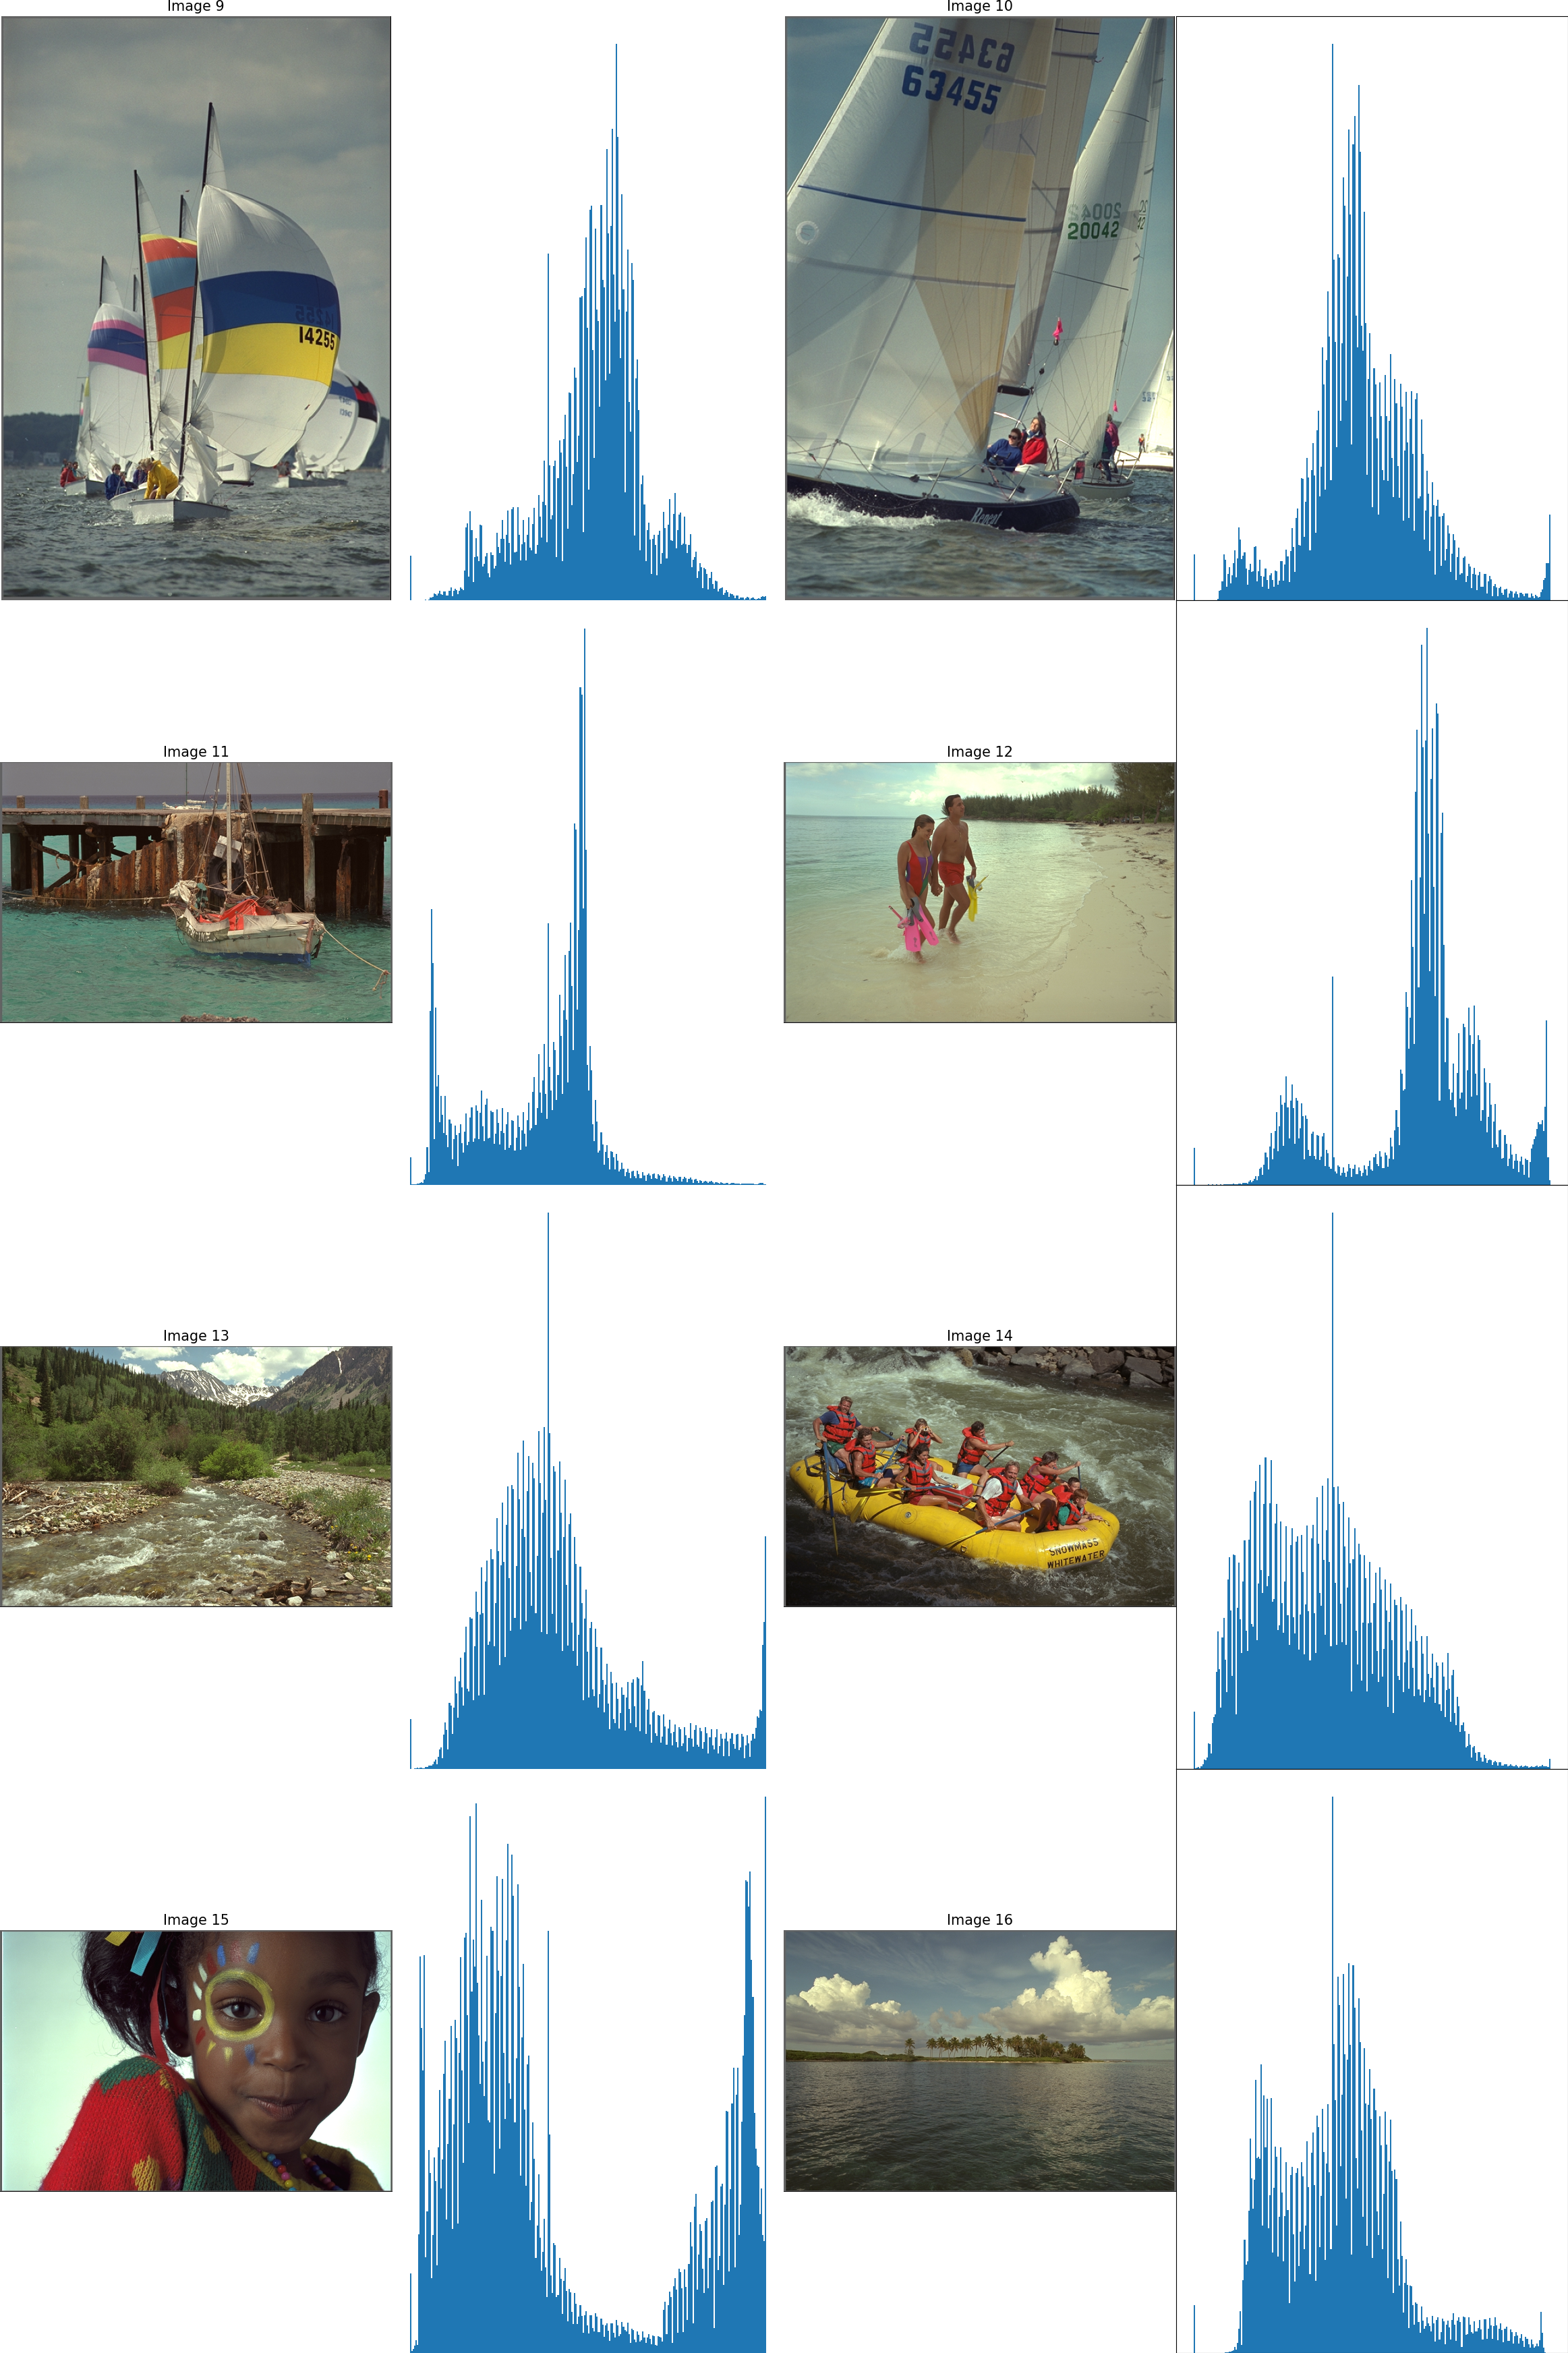
\includegraphics[width=0.8\textwidth]{figuras/img_hist_2.png}
    \caption{Imagen original e histomgrama para todas imagenes del banco, en orden im\'agen 9 hasta 16.}
\end{figure}

\begin{figure}
    \centering
    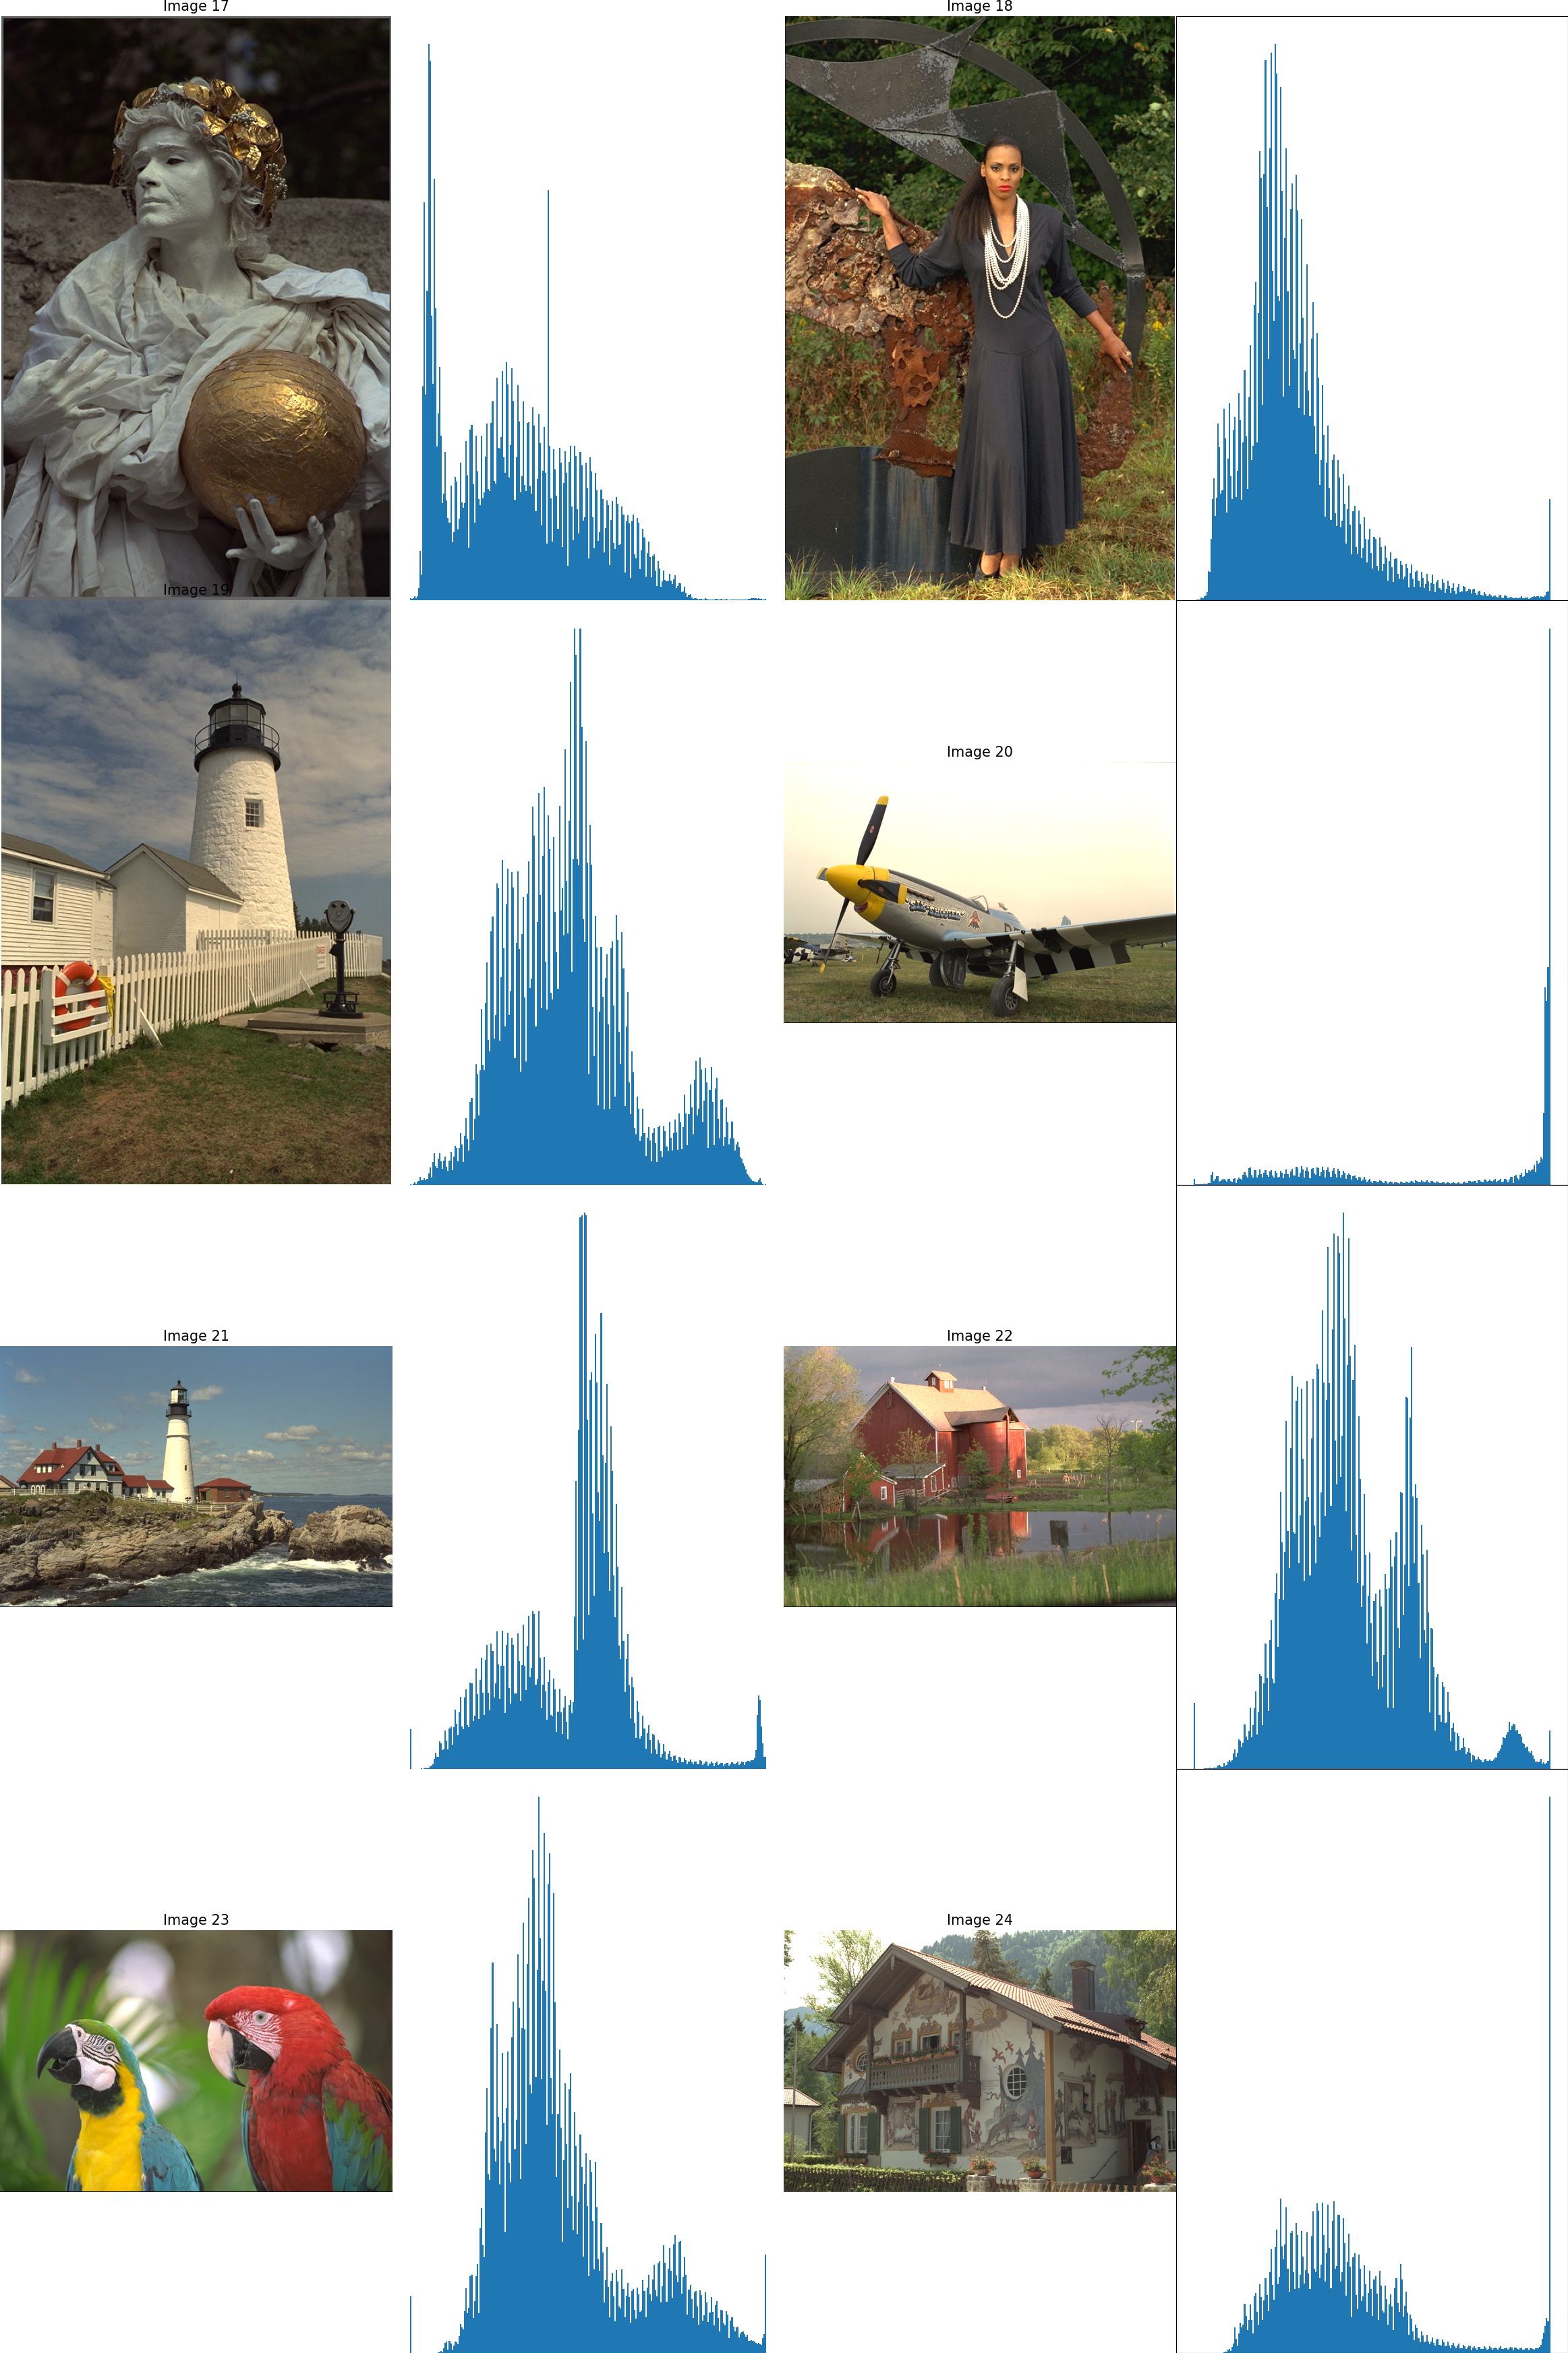
\includegraphics[width=0.8\textwidth]{figuras/img_hist_3.png}
    \caption{Imagen original e histomgrama para todas imagenes del banco, en orden im\'agen 17 hasta 24.}
\end{figure}

\begin{figure}
    \centering
    \includegraphics[width=\textwidth]{figuras/img_hist_noise_1.png}
    \caption{Imagen original junto con su histograma con distintos niveles de ruido, imagenes 1 a 5.}
\end{figure}


\begin{figure}
    \centering
    \includegraphics[width=\textwidth]{figuras/img_hist_noise_2.png}
    \caption{Imagen original junto con su histograma con distintos niveles de ruido, imagenes 6 a 10.}
\end{figure}


\begin{figure}
    \centering
    \includegraphics[width=\textwidth]{figuras/img_hist_noise_3.png}
    \caption{Imagen original junto con su histograma con distintos niveles de ruido, imagenes 11 a 15.}
\end{figure}


\begin{figure}
    \centering
    \includegraphics[width=\textwidth]{figuras/img_hist_noise_4.png}
    \caption{Imagen original junto con su histograma con distintos niveles de ruido, imagenes 16 a 20.}
\end{figure}


\begin{figure}
    \centering
    \includegraphics[width=\textwidth]{figuras/img_hist_noise_5.png}
    \caption{Imagen original junto con su histograma con distintos niveles de ruido, imagenes 21 a 25.}
\end{figure}

\begin{figure}
    \centering
    \includegraphics[width=\textwidth]{figuras/heatmaps/heatmaps_app_0.png}
    \caption{Matriz de calor para las imagenes 1, 2, 3, y 4, cada mapa de calor corresponde a un m\'etodo de comparaci\'on, ya sea comparando el total de la im\'agen (izquierda), o el histograma de estas (derecha). La cantidad de ruido aumenta de izquierda a derecha, y de arriba hacía abajo.}
\end{figure}

\begin{figure}
    \centering
    \includegraphics[width=\textwidth]{figuras/heatmaps/heatmaps_app_1.png}
    \caption{Matriz de calor para las imagenes 5, 6, 7, y 8, cada mapa de calor corresponde a un m\'etodo de comparaci\'on, ya sea comparando el total de la im\'agen (izquierda), o el histograma de estas (derecha). La cantidad de ruido aumenta de izquierda a derecha, y de arriba hacía abajo.}
\end{figure}


\begin{figure}
    \centering
    \includegraphics[width=\textwidth]{figuras/heatmaps/heatmaps_app_2.png}
    \caption{Matriz de calor para las imagenes 9, 10, 11, y 12, cada mapa de calor corresponde a un m\'etodo de comparaci\'on, ya sea comparando el total de la im\'agen (izquierda), o el histograma de estas (derecha). La cantidad de ruido aumenta de izquierda a derecha, y de arriba hacía abajo.}
\end{figure}


\begin{figure}
    \centering
    \includegraphics[width=\textwidth]{figuras/heatmaps/heatmaps_app_3.png}
    \caption{Matriz de calor para las imagenes 13, 14, 15, y 16, cada mapa de calor corresponde a un m\'etodo de comparaci\'on, ya sea comparando el total de la im\'agen (izquierda), o el histograma de estas (derecha). La cantidad de ruido aumenta de izquierda a derecha, y de arriba hacía abajo.}
\end{figure}


\begin{figure}
    \centering
    \includegraphics[width=\textwidth]{figuras/heatmaps/heatmaps_app_4.png}
    \caption{Matriz de calor para las imagenes 17, 18, 19, y 20, cada mapa de calor corresponde a un m\'etodo de comparaci\'on, ya sea comparando el total de la im\'agen (izquierda), o el histograma de estas (derecha). La cantidad de ruido aumenta de izquierda a derecha, y de arriba hacía abajo.}
\end{figure}


\begin{figure}
    \centering
    \includegraphics[width=\textwidth]{figuras/heatmaps/heatmaps_app_5.png}
    \caption{Matriz de calor para las imagenes 21, 22, 23, y 24, cada mapa de calor corresponde a un m\'etodo de comparaci\'on, ya sea comparando el total de la im\'agen (izquierda), o el histograma de estas (derecha). La cantidad de ruido aumenta de izquierda a derecha, y de arriba hacía abajo.}
\end{figure}



\begin{figure}
    \centering
    \includegraphics[width=\textwidth]{figuras/img_BCI_all_1.png}
    \caption{Imagen original junto con sus transformaci\'ones Box-Cox para los distintos m\'etodos de $\lambda$transformados, primera las im\'agenes 1 a 5.}
\end{figure}

\begin{figure}
    \centering
    \includegraphics[width=\textwidth]{figuras/img_BCI_all_2.png}
    \caption{Imagen original junto con sus transformaci\'ones Box-Cox para los distintos m\'etodos de $\lambda$transformados, primera las im\'agenes 6 a 12.}
\end{figure}


\begin{figure}
    \centering
    \includegraphics[width=\textwidth]{figuras/img_BCI_all_3.png}
    \caption{Imagen original junto con sus transformaci\'ones Box-Cox para los distintos m\'etodos de $\lambda$transformados, primera las im\'agenes 13 a 18.}
\end{figure}


\begin{figure}
    \centering
    \includegraphics[width=\textwidth]{figuras/img_BCI_all_4.png}
    \caption{Imagen original junto con sus transformaci\'ones Box-Cox para los distintos m\'etodos de $\lambda$transformados, primera las im\'agenes 19 a 24.}
\end{figure}


\begin{figure}
    \centering
    \includegraphics[width=\textwidth]{figuras/img_BCI_all_1.png}
    \caption{Imagen original junto con sus transformaci\'ones Box-Cox para los distintos m\'etodos de $\lambda$transformados, primera las im\'agenes 1 a 5.}
\end{figure}


\begin{figure}
    \centering
    \includegraphics[width=0.8\textwidth]{figuras/full_comp_1.png}
    \caption{A la izquierda la im\'agen original y a la derecha el valor de $dCor$ (azul), $MIC$ (rojo), y $\rho$ (amarillo) utilizando el vector completo en el eje y, $\lambda$ en el eje x, imagenes 1 a 8.}
\end{figure}

\begin{figure}
    \centering
    \includegraphics[width=0.8\textwidth]{figuras/full_comp_2.png}
    \caption{A la izquierda la im\'agen original y a la derecha el valor de $dCor$ (azul), $MIC$ (rojo), y $\rho$ (amarillo) utilizando el vector completo en el eje y, $\lambda$ en el eje x, imagenes 9 a 16.}
\end{figure}


\begin{figure}
    \centering
    \includegraphics[width=0.8\textwidth]{figuras/full_comp_3.png}
    \caption{A la izquierda la im\'agen original y a la derecha el valor de $dCor$ (azul), $MIC$ (rojo), y $\rho$ (amarillo) utilizando el vector completo en el eje y, $\lambda$ en el eje x, imagenes 17 a 24.}
\end{figure}

\begin{figure}
    \centering
    \includegraphics[width=0.8\textwidth]{figuras/hist_comp_1.png}
    \caption{A la izquierda la im\'agen original y a la derecha el valor de $dCor$ (azul), $MIC$ (rojo), y $\rho$ (amarillo) utilizando el histograma en el eje y, $\lambda$ en el eje x, imagenes 1 a 8.}
\end{figure}

\begin{figure}
    \centering
    \includegraphics[width=0.8\textwidth]{figuras/hist_comp_2.png}
    \caption{A la izquierda la im\'agen original y a la derecha el valor de $dCor$ (azul), $MIC$ (rojo), y $\rho$ (amarillo) utilizando el histograma en el eje y, $\lambda$ en el eje x, imagenes 9 a 16.}
\end{figure}


\begin{figure}
    \centering
    \includegraphics[width=0.8\textwidth]{figuras/hist_comp_3.png}
    \caption{A la izquierda la im\'agen original y a la derecha el valor de $dCor$ (azul), $MIC$ (rojo), y $\rho$ (amarillo) utilizando el histograma en el eje y, $\lambda$ en el eje x, imagenes 17 a 24.}
\end{figure}




% ---------------------------------------------------------------------------------------------
% ---------------------------------------------------------------------------------------
\chapter{C\'odigo.}\label{appB}

En este ap\'endice incluimos una catalogaci\'on de los c\'odigos utilizados para la realizaci\'on de este trabajo. El total de los codigos se encuentra en el repositorio de github \url{https://github.com/FabianCastellano/memoria}, junto con el \LaTeX \ de este documento, y otros archivos de interes. 

\dirtree{%
.1 Repositorio Memoria.
    .2 code.
        .3 boxcox\_comparison\DTcomment{Comparaci\'on de im\'agenes}.
        .3 boxcox\DTcomment{Definicion de Box-Cox y BCI}.
        .3 comparison \DTcomment{Codigo de comparaci\'on de im\'agenes}.
        .3 dCor.\DTcomment{Pruebas de dCor}.
        .3 figuras\DTcomment{Creaci\'on de figuras varias}.
        .3 legacy\DTcomment{C\'odigo no usado en la memoria}.
        .3 MIC\DTcomment{Pruebas del MIC}.
    .2 latexmemoria.
        .3 figuras.
        .3 tesis\_FCN.tex     \DTcomment{Archivo principal donde se unen los Cap\'itulos} .
        .3 \textit{otros}.tex \DTcomment{Capitulos individules}.
    .2 pdfs.
        .3 Correlations\DTcomment{Papers Correspondientes a correlaciones}.
        .3 papers\DTcomment{Otros papers usados y consultados}.
    .2 presentaciones. 
        .3 presentacion\_defensa\DTcomment{Beamer Defensa de T\'itulo}.
        .3 presentacion\_proy\_memo\DTcomment{Beamer presentaci\'ion Proy. de Memoria}.
}
% ---------------------------------------------------------------------------------------
\chapter{Demostraciones}\label{appC}

En este ap\'endice se presentan demostraciones omitidas en al texto principal.
% ---------------------------------------------------------------------------------------------

\blankpage
\printbibliography %Prints bibliography
% --------------------------------------------------
\end{document} 